              %******************************************%
              %                                          %
              % Modello di tesi di laurea o di dottorato %
              %            di Lorenzo Pantieri           %
              %                                          %
              %                © 2013-2017               %
              %                                          %
              %******************************************%
       

% I seguenti commenti speciali impostano:
% 1. utf8 come codifica di input,
% 2. PDFLaTeX come motore di composizione;
% 3. Tesi.tex come documento principale;
% 4. il controllo ortografico italiano per l'editor.

% !TEX encoding = UTF-8 Unicode
% !TEX TS-program = pdflatex
% !TEX root = Tesi.tex
% !TeX spellcheck = <none>

\documentclass[11pt,%                      % corpo del font principale
               a4paper,%                   % carta A4
%              twoside,openright,%         % fronte-retro
               oneside,openany,%           % solo fronte
               titlepage,%                 % frontespizio
               headinclude,,footinclude,%  % testatina e piede di pagina
               BCOR5mm,%                   % rilegatura di 5 mm
               cleardoublepage=empty,%     % pagine vuote senza testatina e piede di pagina
               captions=tableheading,%     % didascalie in cima alle tabelle
               ]{scrreprt}                 % classe report di KOMA-Script;
               
\usepackage[T1]{fontenc}                   % codifica dei font:
                                           % NOTA BENE! richiede una distribuzione *completa* di LaTeX,
                                           % per esempio TeXLive o MiKTeX *complete*

\usepackage[utf8]{inputenc}                % codifica di input; anche [latin1] va bene
                                           % NOTA BENE! va accordata con le preferenze dell'editor

\usepackage[english,italian]{babel}        % per scrivere in italiano e in inglese;
                                           % l'ultima lingua (l'italiano) risulta predefinita

\usepackage[suftesi]{frontespizio}         % frontespizo
                                           % per includerlo nel documento bisogna:
                                           % 1. compilare una prima volta Tesi.tex;
                                           % 2. compilare a parte Tesi-frn.tex, generato dalla compilazione precedente;
                                           % 3. compilare ancora Tesi.tex. 

%\usepackage{indentfirst}                   % rientra il primo capoverso di ogni sezione

\usepackage{graphicx}                      % immagini

\usepackage{listings}                      % codici

\usepackage[font=small]{quoting}           % citazioni

\usepackage{amsmath,amssymb,amsthm}        % matematica

\usepackage[italian]{varioref}             % riferimenti completi della pagina

\usepackage{tabularx}                      % tabelle di larghezza prefissata

\usepackage[autostyle,italian=guillemets]{csquotes} % virgolette ottimizzate per biblatex

\usepackage[style=philosophy-modern,hyperref,square,backend=biber]{biblatex}
                                           % eccellente pacchetto per la bibliografia;
                                           % produce uno stile di citazione autore-anno; 
                                           % lo stile "numeric-comp" produce riferimenti numerici;
                                           % NOTA BENE! bisogna che il proprio editor sia configurato per biber
                                          
\addbibresource{Bibliografia.bib}          % database di biblatex 
                                          
\usepackage{subfig}                        % sottofigure, sottotabelle

\usepackage{lipsum}                        % testo fittizio

\usepackage{eurosym}                       % simbolo dell'euro

\usepackage[eulerchapternumbers,%          % numeri dei capitoli nel font Euler
            subfig,%                       % se si usa il pacchetto subfig
            beramono,%                     % Bera Mono come font a spaziatura fissa
            eulermath,%                    % AMS Euler come font per la matematica
            pdfspacing,%                   % migliora il riempimento di riga
            listings,%                     % codici
%           parts,%                        % da decommentare in un documento diviso in parti
            ]{classicthesis}               % stile ClassicThesis

\usepackage{arsclassica}                   % modifica l'aspetto di ClassicThesis

%*********************************************************************************
% impostazioni-tesi.tex
% di Lorenzo Pantieri (2013-2016)
% file che contiene le impostazioni della tesi
%*********************************************************************************


%*********************************************************************************
% Comandi personali
%*******************************************************
\newcommand{\myName}{Michele Vaccari}                            % autore
\newcommand{\myTitle}{Progetto E-Commerce BINS}                  % titolo
\newcommand{\myDegree}{Documentazione Basi di Dati}   % tipo di tesi
\newcommand{\myUni}{Universit\'a degli Studi di Ferrara}         % universit�
\newcommand{\myFaculty}{Facolt\'a di Ingegneria}                 % facolt\'a
\newcommand{\myDepartment}{Dipartimento di Ingegneria}           % dipartimento
\newcommand{\myProf}{Prof.~Denis~Ferraretti}                      % relatore
%\newcommand{\myOtherProf}{Dott.~Immanuel Kant}                  % correlatore (se presente)
\newcommand{\myLocation}{Castagnaro}                             % dove
\newcommand{\myTime}{Settembre 2017}                             % quando



%*********************************************************************************
% Impostazioni di amsmath, amssymb, amsthm
%*********************************************************************************

% comandi per gli insiemi numerici (serve il pacchetto amssymb)
\newcommand{\numberset}{\mathbb} 
\newcommand{\N}{\numberset{N}} 
\newcommand{\R}{\numberset{R}} 

% un ambiente per i sistemi
\newenvironment{sistema}%
  {\left\lbrace\begin{array}{@{}l@{}}}%
  {\end{array}\right.}

% definizioni (serve il pacchetto amsthm)
\theoremstyle{definition} 
\newtheorem{definizione}{Definizione}

% teoremi, leggi e decreti (serve il pacchetto amsthm)
\theoremstyle{plain} 
\newtheorem{teorema}{Teorema}
\newtheorem{legge}{Legge}
\newtheorem{decreto}[legge]{Decreto}
\newtheorem{murphy}{Murphy}[section]



%*********************************************************************************
% Impostazioni di biblatex
%*********************************************************************************
\defbibheading{bibliography}{%
\cleardoublepage
\manualmark
\phantomsection 
\addcontentsline{toc}{chapter}{\tocEntry{\bibname}}
\chapter*{\bibname\markboth{\spacedlowsmallcaps{\bibname}}
{\spacedlowsmallcaps{\bibname}}}}



%*********************************************************************************
% Impostazioni di listings
%*********************************************************************************
\lstset{language=SQL,%[LaTeX]Tex,C++,
    keywordstyle=\color{RoyalBlue},%\bfseries,
    basicstyle=\small\ttfamily,
    %identifierstyle=\color{NavyBlue},
    commentstyle=\color{Green}\ttfamily,
    stringstyle=\rmfamily,
    numbers=none,%left,%
    numberstyle=\scriptsize,%\tiny
    stepnumber=5,
    numbersep=8pt,
    showstringspaces=false,
    breaklines=true,
    frameround=ftff,
    frame=single
} 



%*********************************************************************************
% Impostazioni di hyperref (decommenta le seguenti righe se non carichi arsclassica)
%*********************************************************************************
%\hypersetup{%
%    hyperfootnotes=false,pdfpagelabels,
%    %draft,	% = elimina tutti i link (utile per stampe in bianco e nero)
%    colorlinks=true, linktocpage=true, pdfstartpage=1, pdfstartview=FitV,%
%    % decommenta la riga seguente per avere link in nero (per esempio per la stampa in bianco e nero)
%    %colorlinks=false, linktocpage=false, pdfborder={0 0 0}, pdfstartpage=1, pdfstartview=FitV,% 
%    breaklinks=true, pdfpagemode=UseNone, pageanchor=true, pdfpagemode=UseOutlines,%
%    plainpages=false, bookmarksnumbered, bookmarksopen=true, bookmarksopenlevel=1,%
%    hypertexnames=true, pdfhighlight=/O,%nesting=true,%frenchlinks,%
%    urlcolor=webbrown, linkcolor=RoyalBlue, citecolor=webgreen, %pagecolor=RoyalBlue,%
%    %urlcolor=Black, linkcolor=Black, citecolor=Black, %pagecolor=Black,%
%    pdftitle={\myTitle},%
%    pdfauthor={\textcopyright\ \myName, \myUni, \myFaculty},%
%    pdfsubject={},%
%    pdfkeywords={},%
%    pdfcreator={pdfLaTeX},%
%    pdfproducer={LaTeX with hyperref and ClassicThesis}%
%}



%*********************************************************************************
% Impostazioni di graphicx
%*********************************************************************************
\graphicspath{{immagini/}} % cartella dove sono riposte le immagini



%*********************************************************************************
% Margini ottimizzati per l'A4
%*********************************************************************************
\areaset[current]{370pt}{750pt}
\setlength{\marginparwidth}{7em}
\setlength{\marginparsep}{2em}%



%*********************************************************************************
% Impostazioni di varioref
%*********************************************************************************
\makeatletter
\vref@addto\extrasitalian{%
   \def\reftextfaraway#1{a pagina~\pageref{#1}}%
}
\makeatother



%*********************************************************************************
% Altro
%*********************************************************************************

% [...] ;-)
\newcommand{\omissis}{[\dots\negthinspace]}

% eccezioni all'algoritmo di sillabazione
\hyphenation{Fortran ma-cro-istru-zio-ne nitro-idrossil-amminico}

% correzione di un bug di scrreprt nella numerazione delle figure
\renewcommand*{\figureformat}{%
  \figurename~\thefigure%
  %\autodot%
}
\renewcommand*{\tableformat}{%
  \tablename~\thetable%
  %\autodot%
}                  % file con le impostazioni personali


\begin{document}
\pagestyle{scrheadings} 
\pagenumbering{roman}
%******************************************************************
% Materiale iniziale
%******************************************************************
% !TEX encoding = UTF-8
% !TEX TS-program = pdflatex
% !TEX root = ../Tesi.tex
% !TEX spellcheck = it-IT

%*******************************************************
% Frontespizio
%*******************************************************
\begin{frontespizio}
\Preambolo{\usepackage{iwona}} % riga da commentare se non si carica ArsClassica

\Universita{Ferrara}
\Logo{logo-unife}
%\Facolta{Ingegneria}
\Dipartimento{Ingegneria}
\Corso[Laurea Triennale]{Ingegneria Elettronica e Informatica}
\Annoaccademico{2016--2017}
\Titoletto{Documentazione Basi di Dati}
\Titolo{Progetto E-Commerce: \\ BINS}
%\Sottotitolo{Alcune considerazioni mutevoli}
\NCandidato{Studente}
\Candidato[121955]{Michele Vaccari}
\NRelatore{Docente}{}
\Relatore{Prof. Denis Ferraretti}
%\Relatore{Claudio Beccari}
%\Correlatore{Tommaso Gordini}
%\Correlatore{Ivan Valbusa}
\end{frontespizio}
% !TEX encoding = UTF-8
% !TEX TS-program = pdflatex
% !TEX root = ../Tesi.tex
% !TEX spellcheck = it-IT

%*******************************************************
% Colophon
%*******************************************************
\clearpage
\phantomsection
\thispagestyle{empty}

\hfill

\vfill

\noindent\myName: \textit{\myTitle,}
\myDegree,
\textcopyright\ \MakeTextLowercase{\myTime}.

%\lipsum[2]
%% !TEX encoding = UTF-8
% !TEX TS-program = pdflatex
% !TEX root = ../Tesi.tex
% !TEX spellcheck = it-IT

%*******************************************************
% Dedica
%*******************************************************
\cleardoublepage
\phantomsection
\thispagestyle{empty}
\pdfbookmark{Dedica}{Dedica}

\vspace*{3cm}

\begin{center}
Lorem ipsum dolor sit amet, consectetuer adipiscing elit. \\ \medskip
--- Oscar Wilde    
\end{center}

\medskip

\begin{center}
Dedicato a tutti gli appassionati di \LaTeX.
\end{center}
% !TEX encoding = UTF-8
% !TEX TS-program = pdflatex
% !TEX root = ../Tesi.tex
% !TEX spellcheck = it-IT

%*******************************************************
% Indici
%*******************************************************
\cleardoublepage
\pdfbookmark{\contentsname}{tableofcontents}
\setcounter{tocdepth}{2}
\tableofcontents
\markboth{\spacedlowsmallcaps{\contentsname}}{\spacedlowsmallcaps{\contentsname}} 
\clearpage

\begingroup 
    \let\clearpage\relax
    \let\cleardoublepage\relax
    %*******************************************************
    % Elenco delle figure
    %*******************************************************    
    \phantomsection
    \pdfbookmark{\listfigurename}{lof}
    \listoffigures

    \vspace*{8ex}

    %*******************************************************
    % Elenco delle tabelle
    %*******************************************************
    %\phantomsection
    %\pdfbookmark{\listtablename}{lot}
    %\listoftables
       
\endgroup

\cleardoublepage

%% !TEX encoding = UTF-8
% !TEX TS-program = pdflatex
% !TEX root = ../Tesi.tex
% !TEX spellcheck = it-IT

%*******************************************************
% Sommario+Abstract
%*******************************************************
\cleardoublepage
\phantomsection
\pdfbookmark{Sommario}{Sommario}
\begingroup
\let\clearpage\relax
\let\cleardoublepage\relax
\let\cleardoublepage\relax

\chapter*{Sommario}

\lipsum[1]

\vfill

\selectlanguage{english}
\pdfbookmark{Abstract}{Abstract}
\chapter*{Abstract}

\lipsum[2]

\selectlanguage{italian}

\endgroup			

\vfill


%% !TEX encoding = UTF-8
% !TEX TS-program = pdflatex
% !TEX root = ../Tesi.tex
% !TEX spellcheck = it-IT

%*******************************************************
% Ringraziamenti
%*******************************************************
\cleardoublepage
\phantomsection
\pdfbookmark{Ringraziamenti}{ringraziamenti}

\chapter*{Ringraziamenti}

\begin{flushright}{\slshape    
	Lorem ipsum dolor sit amet, consectetuer adipiscing elit. \\
	Ut purus elit, vestibulum ut, placerat ac, adipiscing vitae, felis. \\
	Curabitur dictum gravida mauris.} \\ \medskip
    --- Donald Ervin Knuth
\end{flushright}

\lipsum[1]

\bigskip
 
\noindent\textit{\myLocation, \MakeTextLowercase{\myTime}}
% !TEX encoding = UTF-8
% !TEX TS-program = pdflatex
% !TEX root = ../Tesi.tex
% !TEX spellcheck = it-IT

%*******************************************************
% Introduzione
%*******************************************************
\cleardoublepage
\pdfbookmark{Introduzione}{introduzione}

\chapter*{Introduzione}

BINS (acronimo ricorsivo di "BINS Is Not Shopping") è un applicazione web liberamente disponibile, indicata soprattutto per commercializzare prodotti alimentari. Lo scopo di questo lavoro è di documentare l'applicazione usando l'UML (Unified Model Language).

La documentazione è articolata come segue.

\begin{description}
	
	\item[{\hyperref[cap:specifiche-progetto]{Il primo capitolo}}]
	contiene le specifiche del progetto descrivendo le caratteristiche e le categorie di utenti dell'applicazione.
	
	\item[{\hyperref[cap:diagramma]{Il secondo capitolo}}]
	contiene la descrizione delle singole entità e delle loro associazioni.
	
	\item[{\hyperref[cap:modello-relazionale]{Il terzo capitolo}}]
	spiega l'algoritmo di traduzione utilizzato per passare dal modello E-R al modello relazionale.
	
	\item[{\hyperref[cap:normalizzazione]{Il quarto capitolo}}]
	spiega il procedimento di normalizzazione e i vari test effettuati per certificare il modello relazionale in $3NF$.
	
	\item[{\hyperref[cap:codice-SQL]{Il quinto capitolo}}]
	riporta il codice SQL utilizzato per creare le tabelle che costituiscono la base dati e alcune interrogazioni effettuate.
	
	\item[{\hyperref[cap:interfaccia-grafica]{Il sesto capitolo}}]
	mostra le schermate dell'applicazione suddivise per funzionalità e per tipo di utente.
	
\end{description}

Per il \emph{Presentation Level} si è usato il framework \emph{Bootstrap} sfruttando al meglio il \emph{responsive design} che viene messo a disposizione dal framework. Per quanto riguarda l'usabilità e il design si è scelto l'approccio \emph{mobile first} ma si è anche prestato attenzione all'uso dell'applicazione in modalità desktop.

Per l'application server si è usato \emph{Tomcat} e si è utilizzato il linguaggio di progammazione Java.
Per interfacciare l'application server con il database si è utilizzato JDBC.

Il DBMS utilizzato è \emph{MySQL}.

Di seguito si riporta il diagramma approssimato relativo allo sviluppo del lavoro in termini di tempo attraverso un diagramma di Gantt:
\cleardoublepage
%******************************************************************
% Materiale principale
%******************************************************************
\pagenumbering{arabic}
% !TEX encoding = UTF-8
% !TEX TS-program = pdflatex
% !TEX root = ../Tesi.tex
% !TEX spellcheck = it-IT

%************************************************
\chapter{Specifiche progetto}
\label{cap:specifiche-progetto}
%************************************************

\section{Caratteristiche del sistema}
Si vuole progettare un'applicazione web per la vendita online dei prodotti di un supermercato.
L'applicazione deve avere un front-end multilingue (italiano e inglese).

I prodotti del supermercato sono suddivisi in reparti (ortofrutta, macelleria, accessori per la casa, cura della persona, ecc.) e ogni prodotto può avere una data di scadenza.

L'applicazione web deve avere le seguenti caratteristiche:

\begin{enumerate}
	
	\item
	\label{f-up}
	Possibilità di visualizzare il catalogo dei prodotti, navigabile per reparto, caratteristiche, marchio, ricerca libera, ecc.
	Possibilità di vedere il singolo prodotto con tutti i dettagli;
	
	\item
	\label{ef-up}
	Possibilità di visualizzare la lista delle ricette. Ogni ricetta ha un nome, un autore, un tempo di preparazione, un testo con le specifiche della sua preparazione, una lista di prodotti;
	
	\item
	Possibilità di inserire prodotti nel carrello e di effettuare l'acquisto di più prodotti in diverse quantità.
	Predisporre la gestione dei prezzi, del totale carrello, la gestione della disponibilità di magazzino, impedendo di poter acquistare quantità non disponibili e prodotti scaduti;
	
	\item
	Gestione di una o più shopping list (lista della spesa);
	
	\item
	Possibilità di inserire o selezionare un indirizzo di consegna da una rubrica personale, di simulare il pagamento e di confermare l'ordine;
	
	\item
	Possibilità di visualizzare lo stato dell'ordine e lo storico degli ordini effettuati;
	
	\item
	\label{ef-ur}
	Gestione di coupon o buoni sconto in fase di acquisto, possibilità di visualizzare il tracking dell'ordine in consegna;
	
	\item
	\label{sf-ua}
	Possibilità di gestire il catalogo (inserimento, modifica, blocco prodotti), i reparti, i brand, ecc.
	Possibilità di gestire la disponibilità di magazzino;
	
	\item
	Gestione di prodotti in push (per cui spingere la vendita) con inserimento in una "vetrina in home page" o in un'area promo;
	
	\item
	Possibilità di visualizzare gli utenti, verificare il numero degli ordini per utente, bloccare eventuali utenti, gestire gli altri utenti amministratori;
	
	\item
	Gestione dei coupon o buoni sconto;
	
	\item
	\label{ef-ua}
	Gestione del tracking dell'ordine, con simulazione di tutti i cambi di stato (consegnato al corriere, in viaggio, consegnato al destinatario, ecc.);
	
\end{enumerate}

\section{Utenti del sistema}
Il sistema prevede che le categorie di utenti sia così rappresentata:

\begin{description}
	
	\item[Utenti pubblici] Possono effettuare i punti dal \ref{f-up} al \ref{ef-up} ed eventualmente registrarsi.
	
	\item[Utenti registrati] Possono effettuare i punti dal \ref{f-up} al \ref{ef-ur} compresi.
	
	\item[Amministratori] Possono effettuare i punti dal \ref{sf-ua} al \ref{ef-ua} compresi.
	
\end{description}   % specifiche del progetto
% !TEX encoding = UTF-8
% !TEX TS-program = pdflatex
% !TEX root = ../Tesi.tex
% !TEX spellcheck = it-IT

%************************************************
\chapter{Diagramma E-R}
\label{cap:diagramma}
%************************************************

Una volta analizzate le specifiche del progetto per il quale si vuole realizzare il database, si identificano e si descrivono le singole entità e le loro associazioni.

\section{Descrizione delle entità}
	
	\subsection{Utente}
	
		\begin{figure}[h]
			\centering
			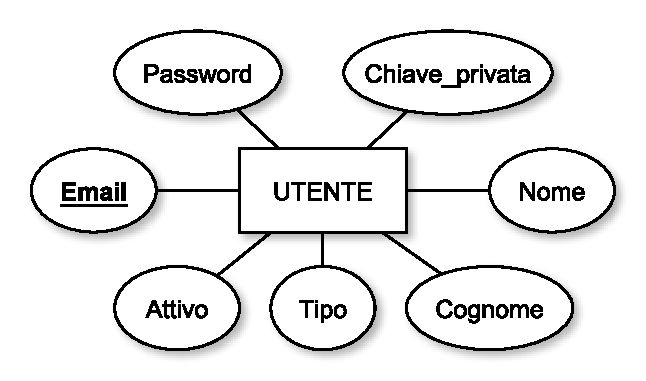
\includegraphics[width=0.5\textwidth]
			{immagini/01-utente}
			
			\caption{Entità Utente}
			\label{entita-utente}
		\end{figure}
		
		Tale entità rappresenta un generico utente dell'applicazione. L'utente si distingue in \emph{Registrato} e \emph{Amministratore}.
		
		La figura \ref{entita-utente} rappresenta l'entità \emph{UTENTE}.
		
		\subsubsection*{Descrizione Attributi}
		
		\begin{description}
			
			\item[Id]
			Chiave primaria dell'entità ``Utente'' che identifica univocamente un utente. Il valore di tale attributo viene assegnato automaticamente dal sistema.
			
			\item[Email]
			Identifica l'email utilizzata dall'utente in fase di autenticazione. Il valore di tale attributo viene inserito dall'utente con relativo controllo di omonimie.
			
			\item[Password]
			Identifica la password utilizzata dall'utente in fase di autenticazione. Il valore di tale attributo viene inserito dall'utente.
			
			\item[Nome]
			Identifica il nome dell'utente con un massimo di 30 caratteri.
			
			\item[Cognome]
			Identifica il cognome dell'utente con un massimo di 30 caratteri.
			
			\item[Tipo]
			Identifica il tipo di utente ovvero:
			\begin{itemize}
				\item
				``A'' per identificare un amministratore;
				\item
				``G'' per identificare il gestore di una squadra;
				\item
				``R'' per identificare un arbitro.
			\end{itemize}
			
			\item[Attivo]
			Identifica lo stato dell'utente, ovvero se è attivo oppure no. Può assumere i valori: ``Y'' oppure ``N''; di default assume valore ``Y'' (attivo).
			
		\end{description}
		
		\subsubsection*{N.B.}
		Nessuno di questi attributi può assumere il valore \texttt{NULL}.
		
		\subsubsection*{Caso Particolare}
		Esiste sempre un valore particolare, ovvero ``admin'', che rappresenta sempre il primo utente Amministratore. Tale valore è sempre presente all'interno della tabella.
	
	\subsection{Amministratore}
	
		\begin{figure}[h]
			\centering
			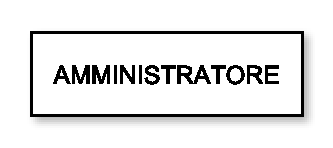
\includegraphics[width=0.3\textwidth]
			{immagini/02-amministratore}
			
			\caption{Entità Amministratore}
			\label{entita-amministratore}
		\end{figure}
		
		Tale entità rappresenta la specializzazione dell'entità \emph{Utente}, ereditandone tutti gli attributi. Serve per rappresentare gli utenti \emph{Amministratori}.
		
		La figura \ref{entita-amministratore} rappresenta l'entità \emph{AMMINISTRATORE}.
	
	\subsection{Registrato}
	
		\begin{figure}[h]
			\centering
			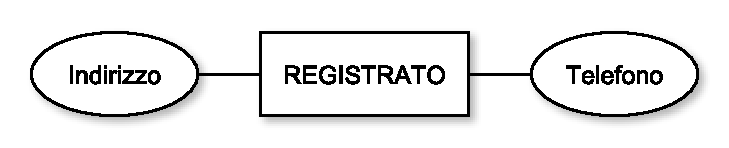
\includegraphics[width=0.6\textwidth]
			{immagini/03-registrato}
			
			\caption{Entità Registrato}
			\label{entita-registrato}
		\end{figure}
		
		Tale entità rappresenta la specializzazione dell'entità \emph{Utente}, ereditandone tutti gli attributi. Serve per rappresentare gli utenti \emph{Gestori Squadra} e gli utenti \emph{Arbitri} che possono accedere all'applicazione Web. Tale entità può essere creata solo dall'amministratore.
		
		La figura \ref{entita-registrato} rappresenta l'entità \emph{REGISTRATO}.
		
		\subsubsection*{Descrizione Attributi}
		
		\begin{description}
			
			\item[Indirizzo]
			Identifica l'indirizzo dell'utente con un massimo di 50 caratteri.
			
			\item[Telefono]
			Identifica il telefono dell'utente con un massimo di 15 caratteri.
			
		\end{description}
		
		\subsubsection*{N.B.}
		Nessuno di questi attributi può assumere il valore \texttt{NULL}.
	
	\subsection{Arbitro}
		
		\begin{figure}[h]
			\centering
			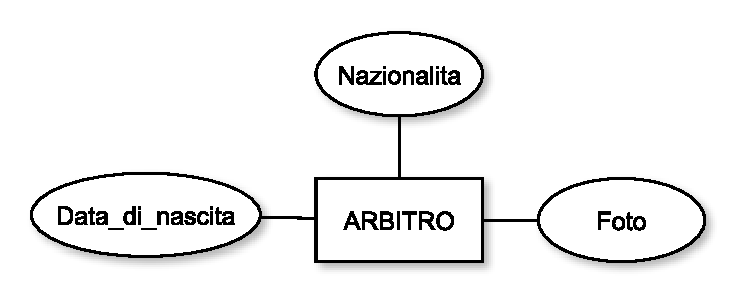
\includegraphics[width=0.6\textwidth]
			{immagini/04-arbitro}
			
			\caption{Entità Arbitro}
			\label{entita-arbitro}
		\end{figure}
		
		Tale entità rappresenta la specializzazione dell'entità \emph{Registrato}, ereditandone tutti gli attributi. Serve per rappresentare il tipo di utente \emph{Arbitro}. Tale entità può essere creata solo dall'amministratore.
		
		La figura \ref{entita-arbitro} rappresenta l'entità \emph{ARBITRO}.
		
		\subsubsection*{Descrizione Attributi}
		
		\begin{description}
			
			\item[Data nascita]
			Identifica la data di nascita dell'utente.
			
			\item[Nazionalita]
			Identifica la nazionalità dell'utente con un massimo di 50 caratteri.
			
			\item[Foto]
			Identifica il percorso dell'immagine all'interno della cartella \emph{Immagini} del server con un massimo di 50 caratteri.
			
			\item[Carriera]
			Campo utilizzato dall'amministratore per inserire delle informazioni aggiuntive relative all'arbitro.
			
		\end{description}
		
		\subsubsection*{N.B.}
		Nessuno di questi attributi può assumere il valore \texttt{NULL}.
	
	\subsection{Gestore Squadra}
	
		\begin{figure}[h]
			\centering
			
\includegraphics[width=0.3\textwidth]
			{immagini/05-gestore-squadra}
			
			\caption{Entità Gestore Squadra}
			\label{entita-gestore-squadra}
		\end{figure}
		
		Tale entità rappresenta la specializzazione dell'entità \emph{Registrato}, ereditandone tutti gli attributi. Serve per rappresentare il tipo di utente \emph{Gestore Squadra}. Tale entità può essere creata solo dall'amministratore.
		
		La figura \ref{entita-gestore-squadra} rappresenta l'entità \emph{GESTORE SQUADRA}.
	
	\subsection{Torneo}
	
		\begin{figure}[h]
			\centering
			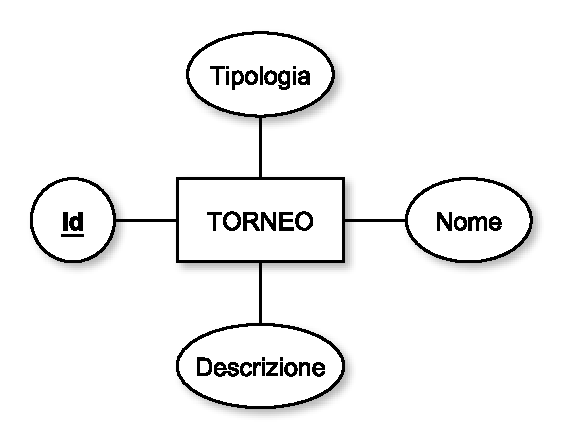
\includegraphics[width=0.5\textwidth]
			{immagini/06-torneo}
			
			\caption{Entità Torneo}
			\label{entita-torneo}
		\end{figure}
		
		Tale entità rappresenta un torneo in svolgimento o già svolto. Può essere di due tipi: ad eliminazione diretta o all'italiana. Tale entità può essere creata solo dall'amministratore.
		
		La figura \ref{entita-torneo} rappresenta l'entità \emph{TORNEO}.
		
		\subsubsection*{Descrizione Attributi}
		
		\begin{description}
			
			\item[Id]
			Chiave primaria dell'entità ``Torneo'' che identifica univocamente un torneo. Il valore di tale attributo viene assegnato automaticamente dal sistema.
			
			\item[Tipologia]
			Identifica la tipologia di torneo ovvero:
			\begin{itemize}
				\item
				``E'' per identificare un torneo ad eliminazione diretta;
				\item
				``I'' per identificare un torneo all'italiana;
			\end{itemize}
			
			\item[Nome]
			Identifica il nome del torneo con un massimo di 30 caratteri.
			
			\item[Descrizione]
			Campo utilizzato dall'amministratore per inserire delle informazioni aggiuntive relative al torneo (storia, luogo, sponsor, ecc.).
			
		\end{description}
		
		\subsubsection*{N.B.}
		Ad eccezione del campo ``Descrizione'', nessuno di questi attributi può assumere il valore \texttt{NULL}.
	
	\subsection{Partita}
		
		\begin{figure}[h]
			\centering
			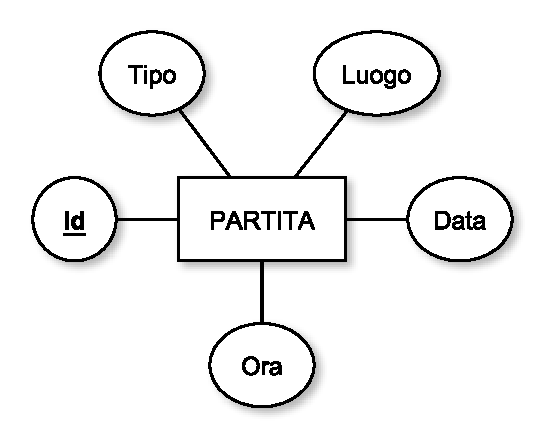
\includegraphics[width=0.5\textwidth]
			{immagini/07-partita}
			
			\caption{Entità Partita}
			\label{entita-partita}
		\end{figure}
		
		Tale entità rappresenta una partita. Tale entità può essere creata solo dall'amministratore.
		
		La figura \ref{entita-partita} rappresenta l'entità \emph{PARTITA}.
		
		\subsubsection*{Descrizione Attributi}
		
		\begin{description}
			
			\item[Id]
			Chiave primaria dell'entità ``Partita'' che identifica univocamente una partita. Il valore di tale attributo viene assegnato automaticamente dal sistema.
			
			\item[Tipo]
			Identifica la tipologia di torneo ovvero:
			\begin{itemize}
				\item
				``E'' per identificare un torneo ad eliminazione diretta;
				\item
				``I'' per identificare un torneo all'italiana;
			\end{itemize}
			Questo attributo serve per gestire in modi diversi le classifiche.
			
			\item[Luogo]
			Identifica il luogo in cui è si svolge la partita con un massimo di 30 caratteri.
			
			\item[Data]
			Identifica la data in cui è si svolge la partita.
			
			\item[Ora]
			Identifica l'ora in cui si svolge la partita.
			
		\end{description}
		
		\subsubsection*{N.B.}
		Nessuno di questi attributi può assumere il valore \texttt{NULL}.
	
	\subsection{Referto}
		
		\begin{figure}[h]
			\centering
			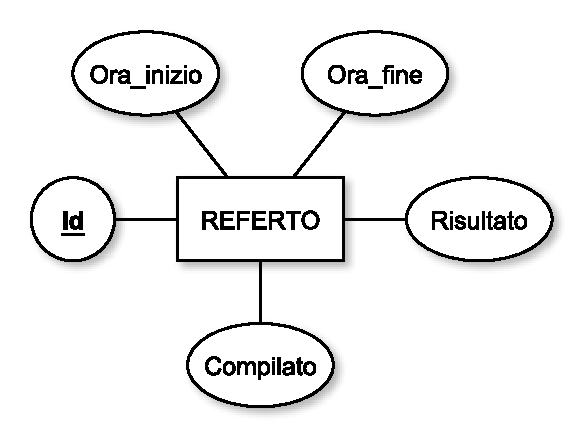
\includegraphics[width=0.5\textwidth]
			{immagini/08-referto}
			
			\caption{Entità Referto}
			\label{entita-referto}
		\end{figure}
		
		Tale entità rappresenta il referto di una determinata gara. Tale entità può essere creata solo dall'arbitro.
		
		La figura \ref{entita-referto} rappresenta l'entità \emph{REFERTO}.
		
		\subsubsection*{Descrizione Attributi}
		
		\begin{description}
			
			\item[Id]
			Chiave primaria dell'entità ``Referto'' che identifica univocamente una partita. Il valore di tale attributo viene assegnato automaticamente dal sistema.
			
			\item[Ora inizio]
			Identifica l'orario effettivo di inizio della partita.
			
			\item[Ora fine]
			Identifica l'orario effettivo di fine della partita.
			
			\item[Risultato]
			Identifica il risultato finale dell'incontro.
			
			\item[Compilato]
			Identifica lo stato del referto, ovvero se è stato compilato oppure no. Può assumere i valori: ``Y'' oppure ``N''; di default assume valore ``N'' (non compilato).
			
		\end{description}
		
		\subsubsection*{N.B.}
		Ad eccezione degli attributi \emph{Ora inizio}, \emph{Ora fine} e \emph{Risultato} tutti gli altri attributi non possono assumere il valore \texttt{NULL}.
	
	\subsection{Squadra}
	
		\begin{figure}[h]
			\centering
			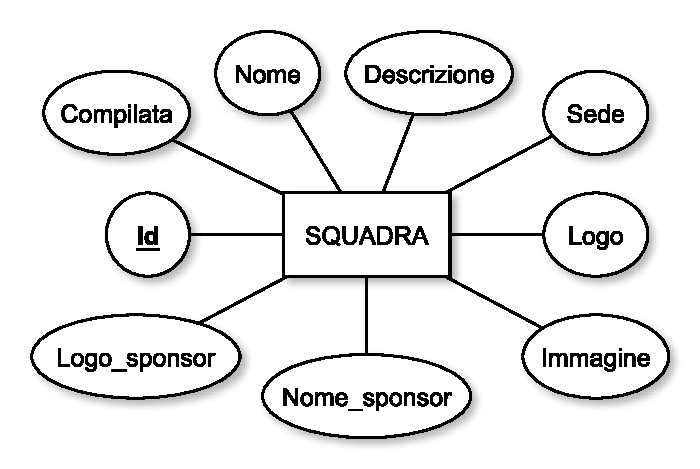
\includegraphics[width=0.6\textwidth]
			{immagini/09-squadra}
			
			\caption{Entità Squadra}
			\label{entita-squadra}
		\end{figure}
		
		Tale entità rappresenta una squadra. Tale entità viene creata dall'amministratore e successivamente viene completata dal gestore della squadra.
		
		La figura \ref{entita-squadra} rappresenta l'entità \emph{SQUADRA}.
		
		\subsubsection*{Descrizione Attributi}
		
		\begin{description}
			
			\item[Id]
			Chiave primaria dell'entità ``Squadra'' che identifica univocamente una partita. Il valore di tale attributo viene assegnato automaticamente dal sistema.
			
			\item[Compilata]
			Identifica lo stato della squadra, ovvero se è stata compilata oppure no. Può assumere i valori: ``Y'' oppure ``N''. Se la squadra non è stata compilata, la prima volta che si accede all'applicazione web si dovranno fornire i dati richiesti. Se non si forniscono i dati della squadra non si può svolgere nessuna attività.
			
			\item[Nome]
			Identifica il nome legale della società con un massimo di 30 caratteri.
			
			\item[Descrizione]
			Campo utilizzato dall gestore della squadra per inserire delle informazioni aggiuntive relative alla squadra.
			
			\item[Sede]
			Identifica la sede legale della società con un massimo di 30 caratteri.
			
			\item[Logo]
			Identifica il percorso del logo della squadra all'interno della cartella \emph{Immagini} del server con un massimo di 50 caratteri.
			
			\item[Immagine]
			Identifica il percorso della foto della squadra all'interno della cartella \emph{Immagini} del server con un massimo di 50 caratteri.
			
			\item[Nome sponsor]
			Identifica il nome dello sponsor ufficiale della squadra con un massimo di 30 caratteri.
			
			\item[Logo sponsor]
			Identifica il percorso del logo dello sponsor all'interno della cartella \emph{Immagini} del server con un massimo di 50 caratteri.
			
		\end{description}
		
		\subsubsection*{N.B.}
		Ad eccezione degli attributi \emph{Id}, \emph{Compilata} e \emph{Nome} tutti gli altri attributi possono assumere il valore \texttt{NULL}.
	
	\subsection{Classifica}
	
		\begin{figure}[h]
			\centering
			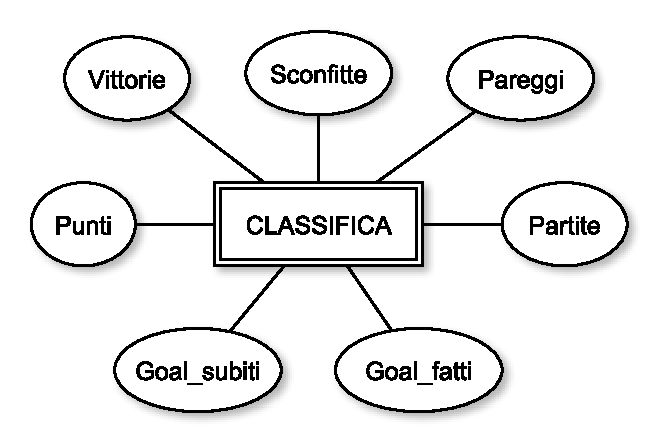
\includegraphics[width=0.6\textwidth]
			{immagini/10-classifica}
			
			\caption{Entità Classifica}
			\label{entita-classifica}
		\end{figure}
		
		Tale entità rappresenta la classifica di un determinato torneo. Tale entità è un'entità debole in quanto non ha propri attributi chiave ma è un torneo ad identificarla univocamente.
		
		La figura \ref{entita-classifica} rappresenta l'entità \emph{CLASSIFICA}.
		
		\subsubsection*{Descrizione Attributi}
		
		\begin{description}
			
			\item[Punti]
			Identifica i punti totalizzati fino a quel momento da una determinata squadra in un determinato torneo.
			
			\item[Vittorie]
			Identifica il numero totale delle partite vinte da una squadra in un determinato torneo.
			
			\item[Sconfitte]
			Identifica il numero totale delle partite perse da una squadra in un determinato torneo.
			
			\item[Pareggi]
			Identifica il numero totale delle partite pareggiate da una squadra in un determinato torneo.
			
			\item[Partite]
			Identifica il numero totale delle partite disputate da una squadra in un determinato torneo.
			
			\item[Goal fatti]
			Identifica il totale dei goal fatti dai giocatori di una determinata squadra in un torneo.
			
			\item[Goal subiti]
			Identifica il totale dei goal subiti dai giocatori una determinata squadra in un torneo.
			
		\end{description}
		
		\subsubsection*{N.B.}
		Nessuno di questi attributi può assumere il valore \texttt{NULL}.
		
	\subsection{Giocatore}
	
		\begin{figure}[h]
			\centering
			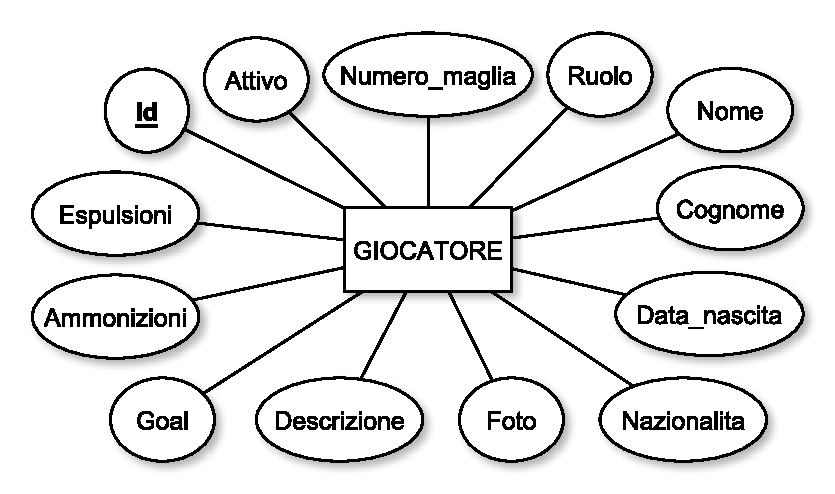
\includegraphics[width=0.8\textwidth]
			{immagini/11-giocatore}
			
			\caption{Entità Giocatore}
			\label{entita-giocatore}
		\end{figure}
		
		Tale entità rappresenta la un determinato giocatore di una squadra.
		
		La figura \ref{entita-giocatore} rappresenta l'entità \emph{GIOCATORE}.
		
		\subsubsection*{Descrizione Attributi}
		
		\begin{description}
			
			\item[Id]
			Chiave primaria dell'entità ``Giocatore'' che identifica univocamente un giocatore. Il valore di tale attributo viene assegnato automaticamente dal sistema.
			
			\item[Attivo]
			Identifica lo stato del giocatore, ovvero se è attivo oppure no. Può assumere i valori: ``Y'' oppure ``N''; di default assume valore ``Y'' (attivo).
			
			\item[Numero maglia]
			Identifica il numero maglia con cui il giocatore prende parte alle partite.
			
			\item[Ruolo]
			Identifica il ruolo che il giocatore interpreta in campo con un massimo di 50 caratteri.
			
			\item[Nome]
			Identifica il nome del giocatore con un massimo di 30 caratteri.
			
			\item[Cognome]
			Identifica il cognome del giocatore con un massimo di 30 caratteri.
			
			\item[Data nascita]
			Identifica la data di nascita del giocatore.
			
			\item[Nazionalita]
			Identifica il nome del giocatore con un massimo di 20 caratteri.
			
			\item[Foto]
			Identifica il percorso della foto del giocatore all'interno della cartella \emph{Immagini} del server con un massimo di 50 caratteri.
			
			\item[Descrizione]
			Campo utilizzato dal gestore della squadra per inserire delle informazioni aggiuntive relative al giocatore.
			
			\item[Goal]
			Indica il numero di goal effettuati dal giocatore.
			
			\item[Ammonizioni]
			Indica il numero di ammonizioni del giocatore.
			
			\item[Espulsioni]
			Indica il numero di espulsioni del giocatore.
			
		\end{description}
		
		\subsubsection*{N.B.}
		Nessuno di questi attributi può assumere il valore \texttt{NULL}.

\section{Descrizione delle associazioni}
	
	\subsection{Ha}
	Associazione presente tra Torneo e Classifica. \\
	L’entità classifica è debole e, per questo motivo, viene rappresentata all'interno di un doppio rettangolo; anche il rombo che rappresenta l'associazione è doppio per lo stesso motivo. 
	Un entità è debole se non ha attributi chiave; tali entità hanno sempre un vincolo di partecipazione totale perché altrimenti non sarebbero identificabili. Come si può notare è presente un vincolo di partecipazione totale dalla parte di classifica.
	La molteplicità è $1:N$ in quanto ad un torneo sono associate più classifiche (una per ogni squadra), ma una classifica può essere associata soltanto ad un singolo torneo.
	
	\subsection{Presente}
	Associazione presente tra Squadra e Classifica. \\
	Valgono le stesse considerazioni fatte per la relazione ``Ha''.
	La molteplicità è $1:N$ in quanto ad una squadra possono essere associate più classifiche (una per ogni torneo a cui la squadra partecipa), ma una classifica può essere associata soltanto ad una squadra.
	
	\subsection{Composta}
	Associazione presente tra Squadra e Giocatore. \\
	Indica quali sono i giocatori che compongono una determinata squadra. In una squadra possono prendere parte al massimo $36$ giocatori. Un giocatore può far parte di una sola squadra. La molteplicità è $1: 36$.
	I $36$ giocatori sono la rosa della squadra.
	
	\subsection{Gestisce}
	Associazione presente tra Gestore Squadra e Squadra. \\
	Identifica chi è il gestore di una determinata squadra. È presente un vincolo di partecipazione totale dalla parte di squadra in quanto non può esistere una squadra se non esiste un gestore che la crea.
	La molteplicità è $1:1$ in quanto una squadra può essere gestita da un solo gestore e viceversa.
	
	\subsection{Riferito}
	Associazione presente tra Partita e Referto. \\
	Serve per associare un referto ad una determinata partita che, deve essere o è già stata, giocata.
	È presente un vincolo di partecipazione totale dalla parte di referto in quanto non esiste un referto se non esiste una partita. 
	La molteplicità è $1:1$ poiché ad una determinata partita è associato un solo referto e viceversa.
	
	\subsection{Gestisce Registrato}
	Associazione presente tra Registrato e Amministratore. \\
	Un registrato (Arbitro e Gestore squadra) deve essere creato da uno degli amministratori. Per questo motivo è presente un vincolo di partecipazione totale dalla parte di registrato. Un registrato non può esistere se non è presente un amministratore che lo abbia creato.
	La molteplicità è $1:N$ in quanto un amministratore può creare più utenti registrati, ma un utente registrato può essere creato da un solo amministratore.
	
	\subsection{Gestisce Torneo}
	Associazione presente tra Amministratore e Torneo. \\
	L’amministratore è l’unico a poter creare un torneo (ad Eliminazione diretta o all'Italiana). Per questo motivo è presente un vincolo di partecipazione totale dalla parte di torneo. Un torneo non può esistere se non c’è un amministratore che lo abbia creato.
	La molteplicità è $1:N$ in quanto un amministratore può creare molti tornei, ma un torneo può essere creato da un solo amministratore.
	
	\subsection{Compila}
	Associazione presente tra Arbitro e Referto. \\
	L'arbitro, scelto da un amministratore per una partita, sarà colui che compilerà il referto della partita.
	È presente un vincolo di partecipazione totale dalla parte di referto, in quanto questo non può esistere se non è esiste un arbitro che può compilare tale referto.
	La molteplicità è $1:N$ in quanto un arbitro può compilare $N$ referti ma un solo referto può essere compilato da un solo Arbitro.
	
	\subsection{Partecipa}
	Associazione presente tra Torneo e Squadra. \\
	Indica a quali tornei partecipano le squadre e quali squadre partecipano ad un determinato torneo.
	La partecipazione totale è dalla parte di Torneo perché non può esistere un Torneo se non sono presenti delle squadre che vi possano partecipare.
	La molteplicità è $M:N$ in quanto una squadra può partecipare a più tornei e un torneo può avere più squadre che vi partecipano, con un minimo di $2$ per un torneo ad eliminazione diretta e con un minimo di $4$ per un torneo all'italiana.
	
	\subsection{Cartellino}
	Associazione presente tra Arbitro e Giocatore. \\
	Indica chi sono i giocatori che hanno avuto un ammonizione o un'espulsione dall'arbitro.
	Tale associazione presenta l’attributo \emph{Numero} che specifica il numero di cartellini gialli assegnati ad un giocatore, l'attributo \emph{Ammonizione} che specifica se un giocatore è stato ammonito oppure no e l'attributo \emph{Espulsione} che specifica se un giocatore è stato espulso oppure no.
	La partecipazione parziale da entrambi i lati perché può esistere un arbitro che non ha mai assegnato un ammonizione o un'espulsione e, viceversa, un giocatore con nessuna ammonizione o espulsione da parte di un arbitro.
	La molteplicità è $M:N$ in quanto un arbitro può ammonire ed espellere più di un giocatore e viceversa.
	
	\subsection{Marcatore}
	Associazione presente tra Referto e Giocatore. \\
	Indica chi sono i giocatori che hanno segnato un goal in un referto.
	Tale associazione presenta l’attributo \emph{Goal} che specifica il numero di goal effettuati da un giocatore.
	La partecipazione parziale in entrambe le parti perché può esistere un referto con nessun giocatore che ha segnato un goal.
	La molteplicità è $M:N$ perché per ogni referto un giocatore segna dei goal e, viceversa, ogni giocatore può segnare dei goal in più referti.
	
	\subsection{Scelto}
	Associazione ternaria presente tra Arbitro, Amministratore e Partita. \\
	Indica che un determinato arbitro è stato scelto da un determinato amministratore per una specifica partita.
	Un arbitro può essere scelto per $N$ diverse partite e per ogni partita è scelto un singolo arbitro. Un amministratore può scegliere $1$ arbitro per una delle $N$ partite, ovvero un arbitro può arbitrare solo una singola partita.
	
	\subsection{Formazione}
	Associazione ternaria presente tra Squadra, Giocatore e Referto. \\
	Serve per sapere chi sono i giocatori titolari e chi sono le riserve che faranno parte alla formazione di una determinata partita.
	Nell'associazione è presente l'attributo \emph{Riserva} che indica se un giocatore è una riserva oppure no.
	Se l'attributo \emph{Riserva} è uguale a ``Y'' allora il giocatore scelto sarà una riserva, in caso sia ``N'' il giocatore sarà un titolare.
	Per ogni referto sono fornite due formazioni, una per ogni squadra, composte da 18 giocatori ($11$ titolari e $7$ riserve).
	
	\subsection{Giocano}
	Associazione ternaria presente tra Partita, Torneo e Squadra. \\
	Indica quali squadre di un determinato torneo si devono affrontare. Tale associazione presenta l’attributo \emph{Numero\_giornata\_o\_fase} che specifica il numero della fase o il numero della giornata dei tornei rispettivamente ad eliminazione diretta o all'italiana. Una partita di un torneo viene giocata sempre da $2$ squadre e, in un torneo, sono possibili $N$ partite. È presente un vincolo di partecipazione totale dalla parte di partita in quanto una partita non può esistere se non è stato creato un torneo o non sono presenti delle squadre.
	

\section{Il modello E-R completo}
Per il modello E-R completo si veda la figura \vref{fig-modello-ER}.


\begin{figure}[h]
	\centering
	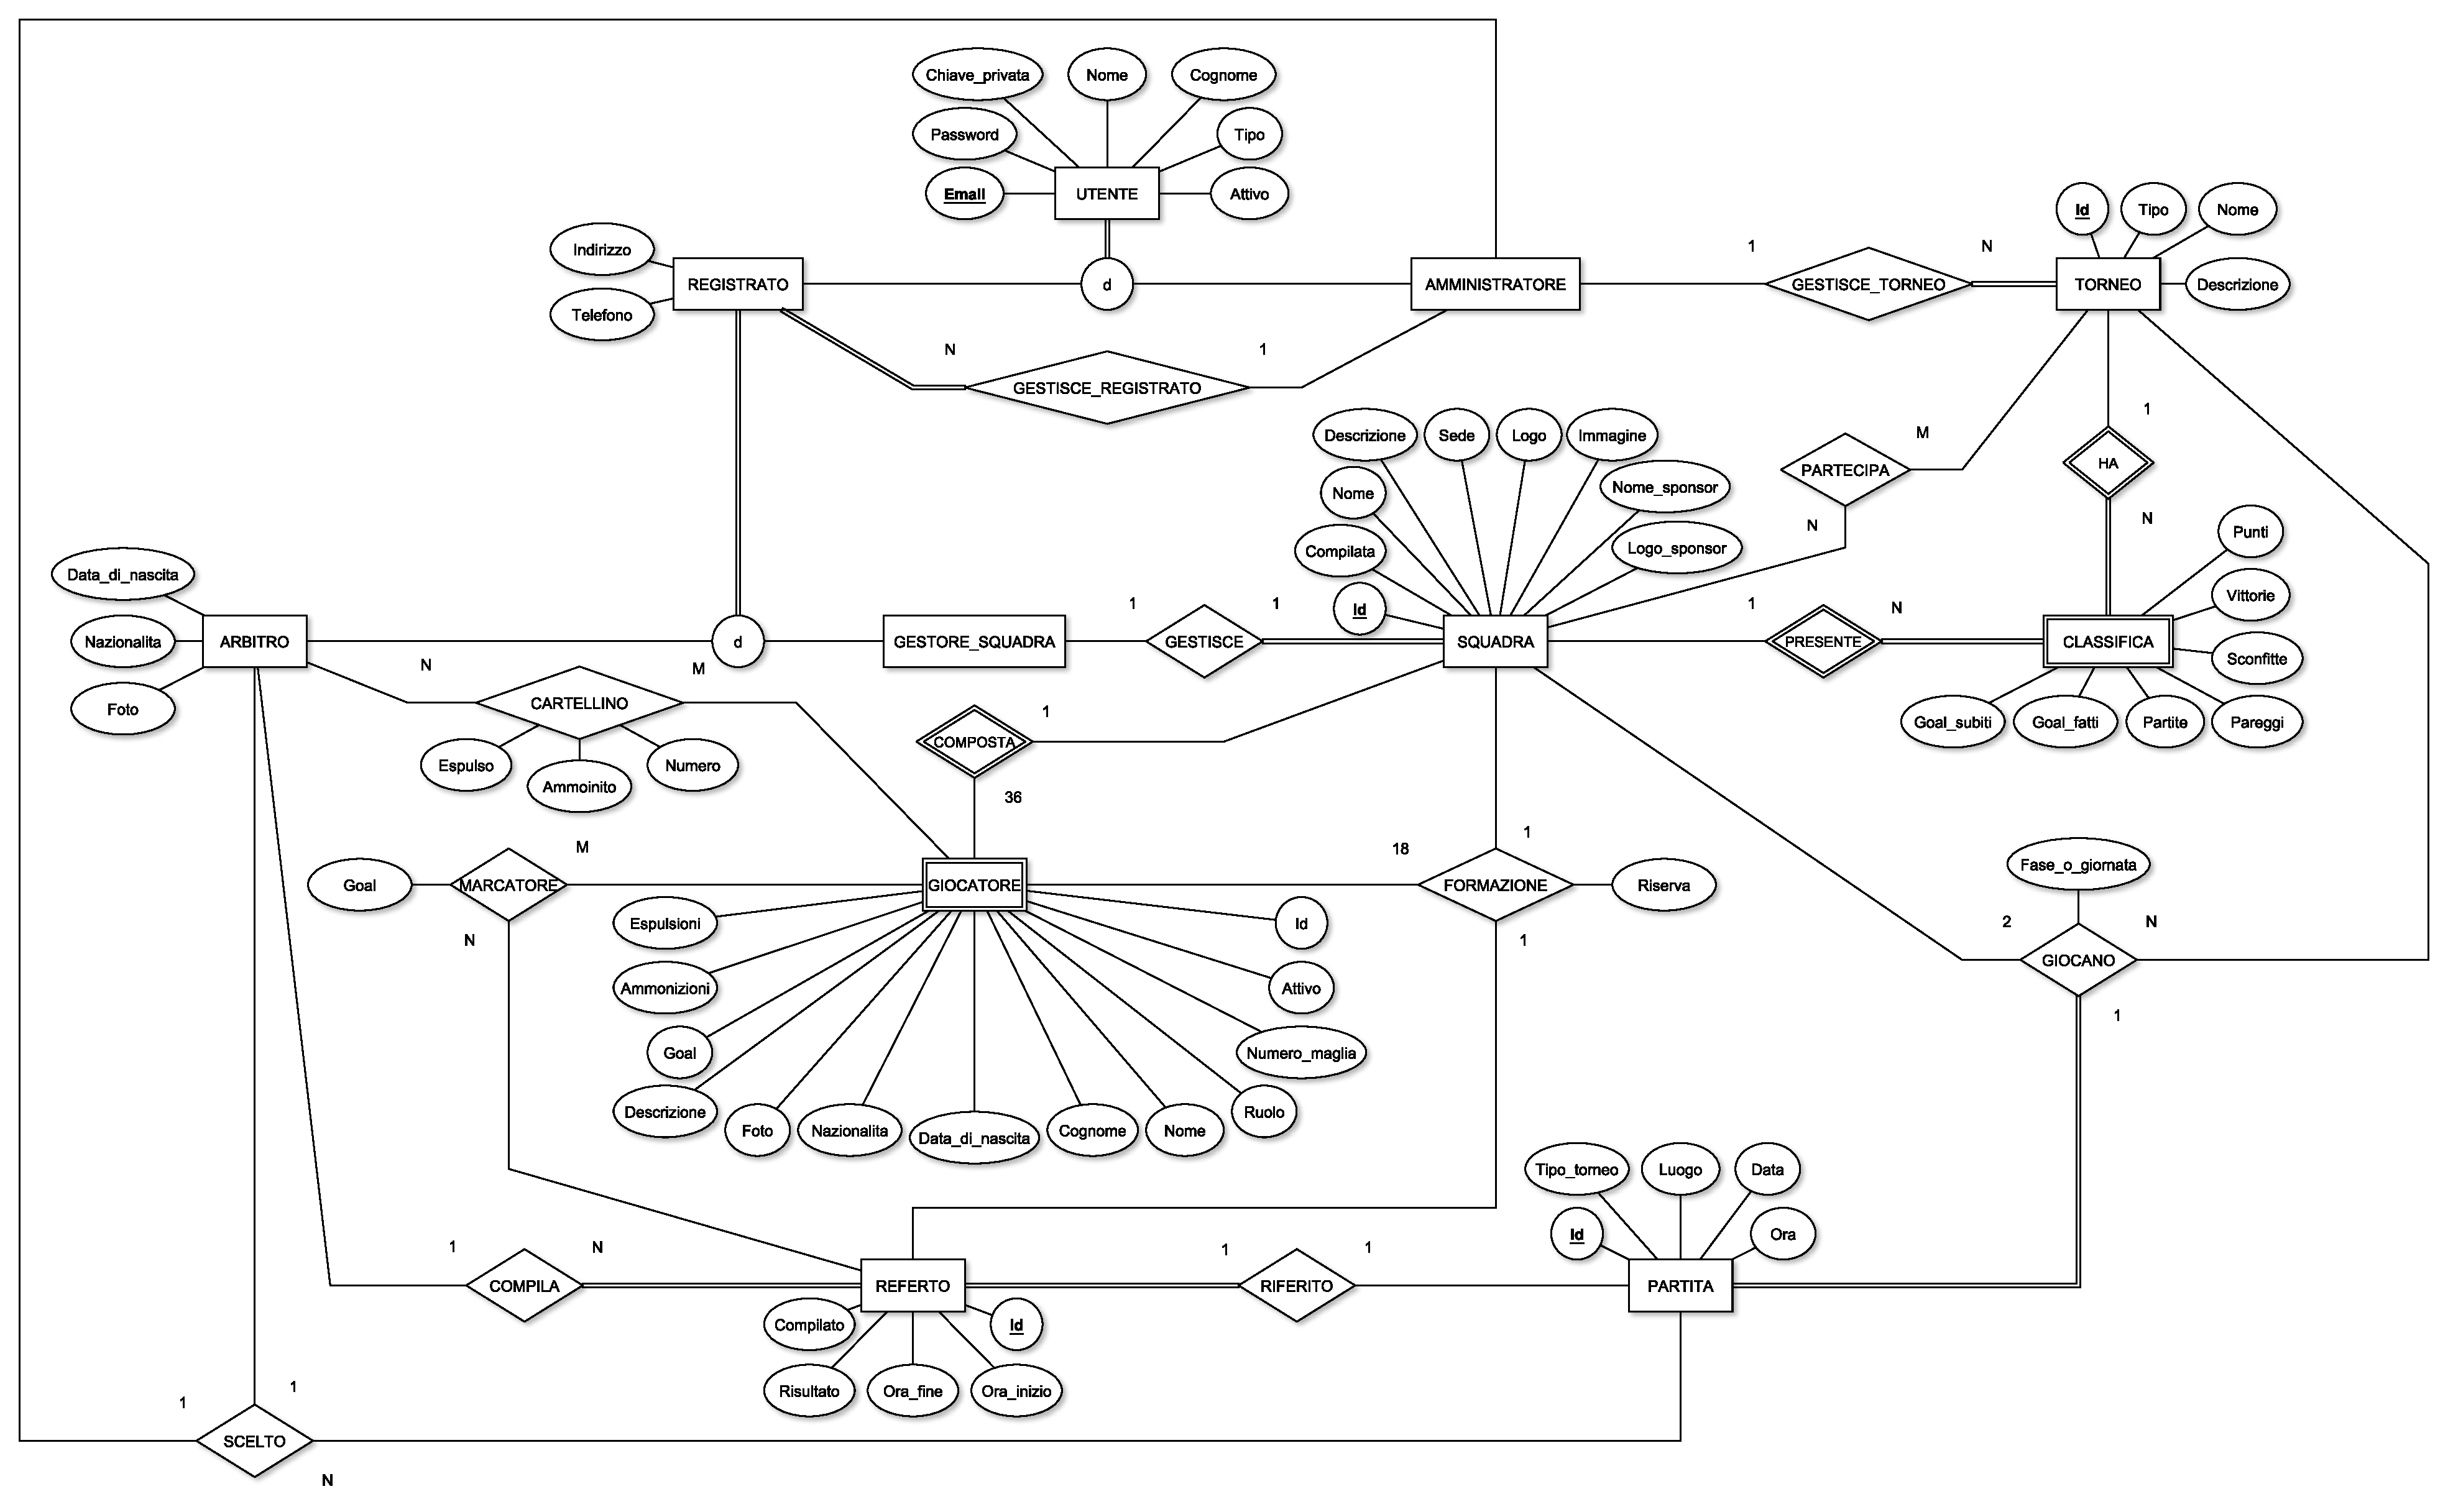
\includegraphics[height=1\textwidth,
	angle=90]
	{immagini/diagramma-ER-completo}
	
	\caption{Schema E-R completo}
	
	\label{fig-modello-ER}
\end{figure}	   % progettazione del diagramma ER
% !TEX encoding = UTF-8
% !TEX TS-program = pdflatex
% !TEX root = ../Tesi.tex
% !TEX spellcheck = it-IT

%************************************************
\chapter{Modello relazionale}
\label{cap:modello-relazionale}
%************************************************

\section{L'algoritmo di traduzione}
La fase successiva della progettazione di una base di dati consiste nel passare dalla progettazione concettuale alla progettazione logica. Per passare al modello relazionale, si applica un semplice algoritmo.

L'algoritmo che si utilizza per la traduzione dal modello E-R in modello relazionale è formato dalle seguenti operazioni:

\begin{enumerate}
	
	\item
	Traduzione di tipi di entità;
	
	\item
	Traduzione di tipi di entità deboli;
	
	\item
	Traduzione di associazioni binarie di tipo $1:1$;
	
	\item
	Traduzione di associazioni binarie di tipo $1:N$;
	
	\item
	Traduzione di associazioni binarie di tipo $N:M$;

\end{enumerate}

\subsection{Traduzione di entità}
	Per ogni tipo di entità (forte) nello schema E-R si costruisce una relazione che contiene tutti gli attributi semplici dell'entità.

\subsection{Traduzione di entità deboli}
	Per ogni tipo di entità debole dello schema E-R con tipo di entità proprietario, si costruisce una relazione e si inseriscono tutti gli attributi semplici dell'entità debole come attributi della relazione. Si inseriscono come attributi di chiave esterna della relazione gli attributi di chiave primaria delle relazioni corrispondenti ai tipi di entità proprietari. La chiave primaria della relazione è data dalla combinazione delle chiavi primarie delle entità proprietarie e dalla chiave parziale del tipo di entità debole (se esiste).

\subsection{Traduzione di associazioni binarie 1:1}
	Per ogni tipo di associazione binaria $1:1$ nello schema E-R si individuano le due relazioni coinvolte dall'associazione. Per la traduzione si usa l'approccio basato su chiavi esterne. Si seglie una delle due relazioni coinvolte, preferibilmente la relazione corrispondente a un tipo di entità con vincolo di partecipazione totale, e si inserisce come chiave esterna la chiave primaria della seconda relazione. Infine si inseriscono sulla relazione scelta tutti gli attributi semplici del tipo di associazione $1:1$.

\subsection{Traduzione di associazioni binarie 1:N}
	Per ogni tipo di associazione binaria $1:N$ nello schema E-R si individuano le due relazioni coinvolte dall'associazione. Per la traduzione si individuata la relazione che rappresenta il tipo di entità partecipante lato-N del tipo di associazione e si inserisce come chiave esterna la chiave primaria della relazione che rappresenta l'altro tipo di entità partecipante all'associazione. Infine si inseriscono sulla relazione scelta tutti gli attributi semplici del tipo di associazione $1:N$.

\subsection{Traduzione di associazioni binarie N:M}
	Per ogni tipo di associazione binaria $M:N$ nello schema E-R si costruisce una nuova relazione che rappresenta l'associazione. Si inseriscono come attributi di chiave esterna della relazione le chiavi primarie delle relazioni che rappresentano i tipi di entità partecipanti, le loro combinazioni formano la chiave primaria della relazione. Infine si inseriscono nella nuova relazione tutti gli attributi semplici del tipo di associazione $M:N$.

\section{Applicazione dell'algoritmo di traduzione}
	Di seguito si riporta la traduzione in modello relazionale del modello E-R analizzato:
	
	\begin{figure}[h]
		\centering
		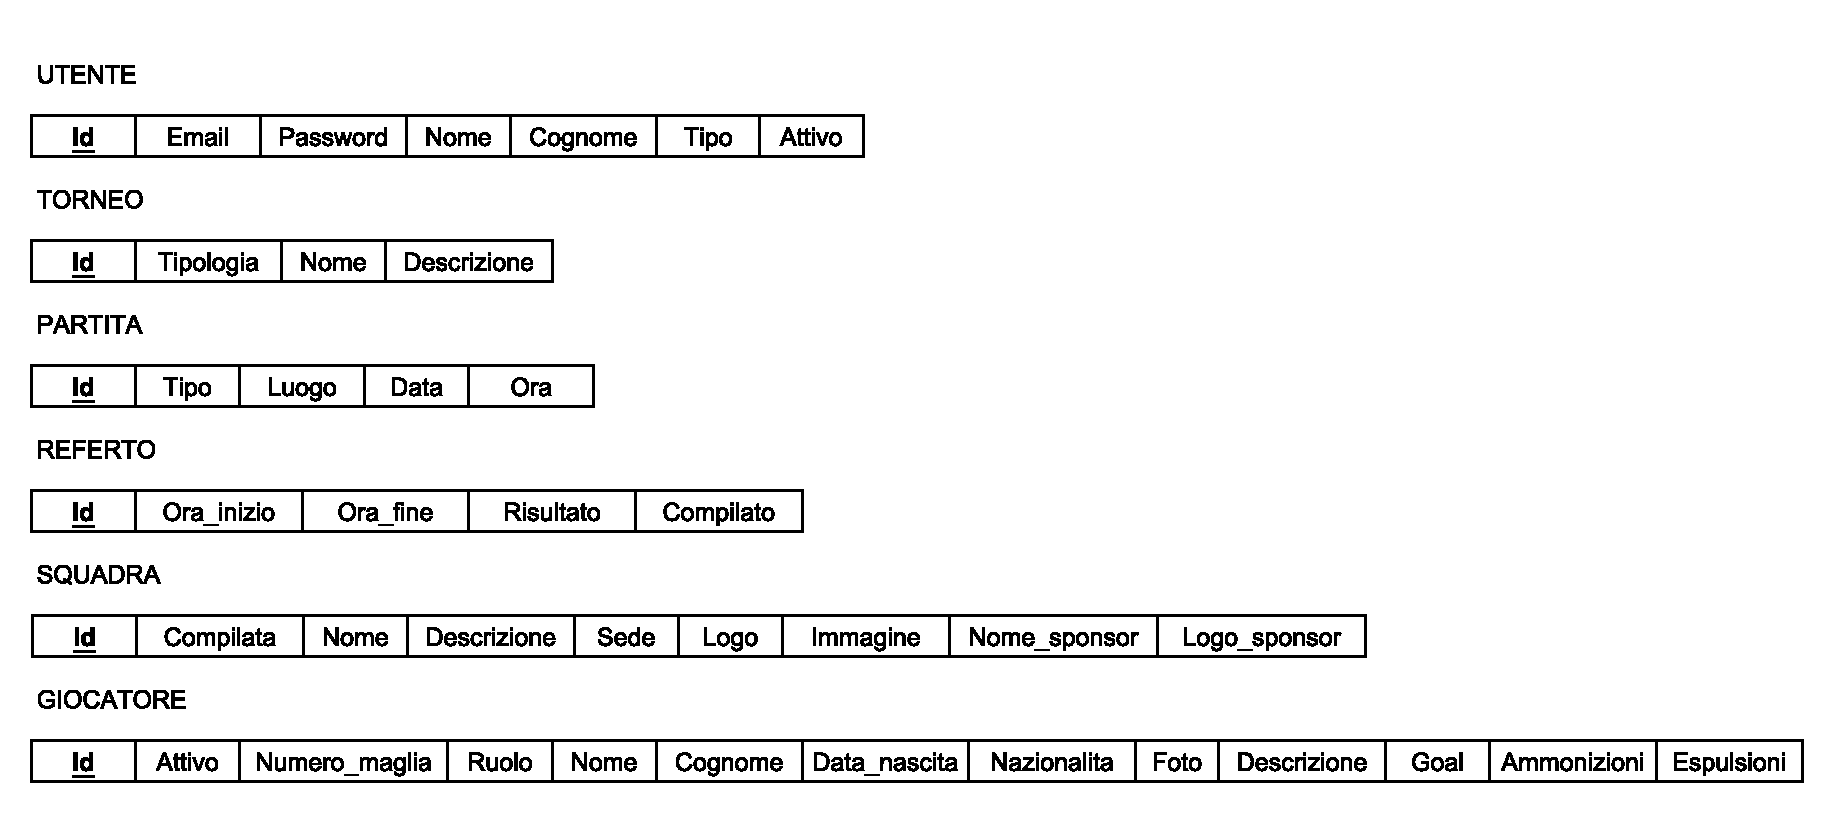
\includegraphics[width=1\textwidth]
		{immagini/traduzione-entita}
		
		\caption{Traduzione di entità}
	\end{figure}
	
	\begin{figure}[h]
		\centering
		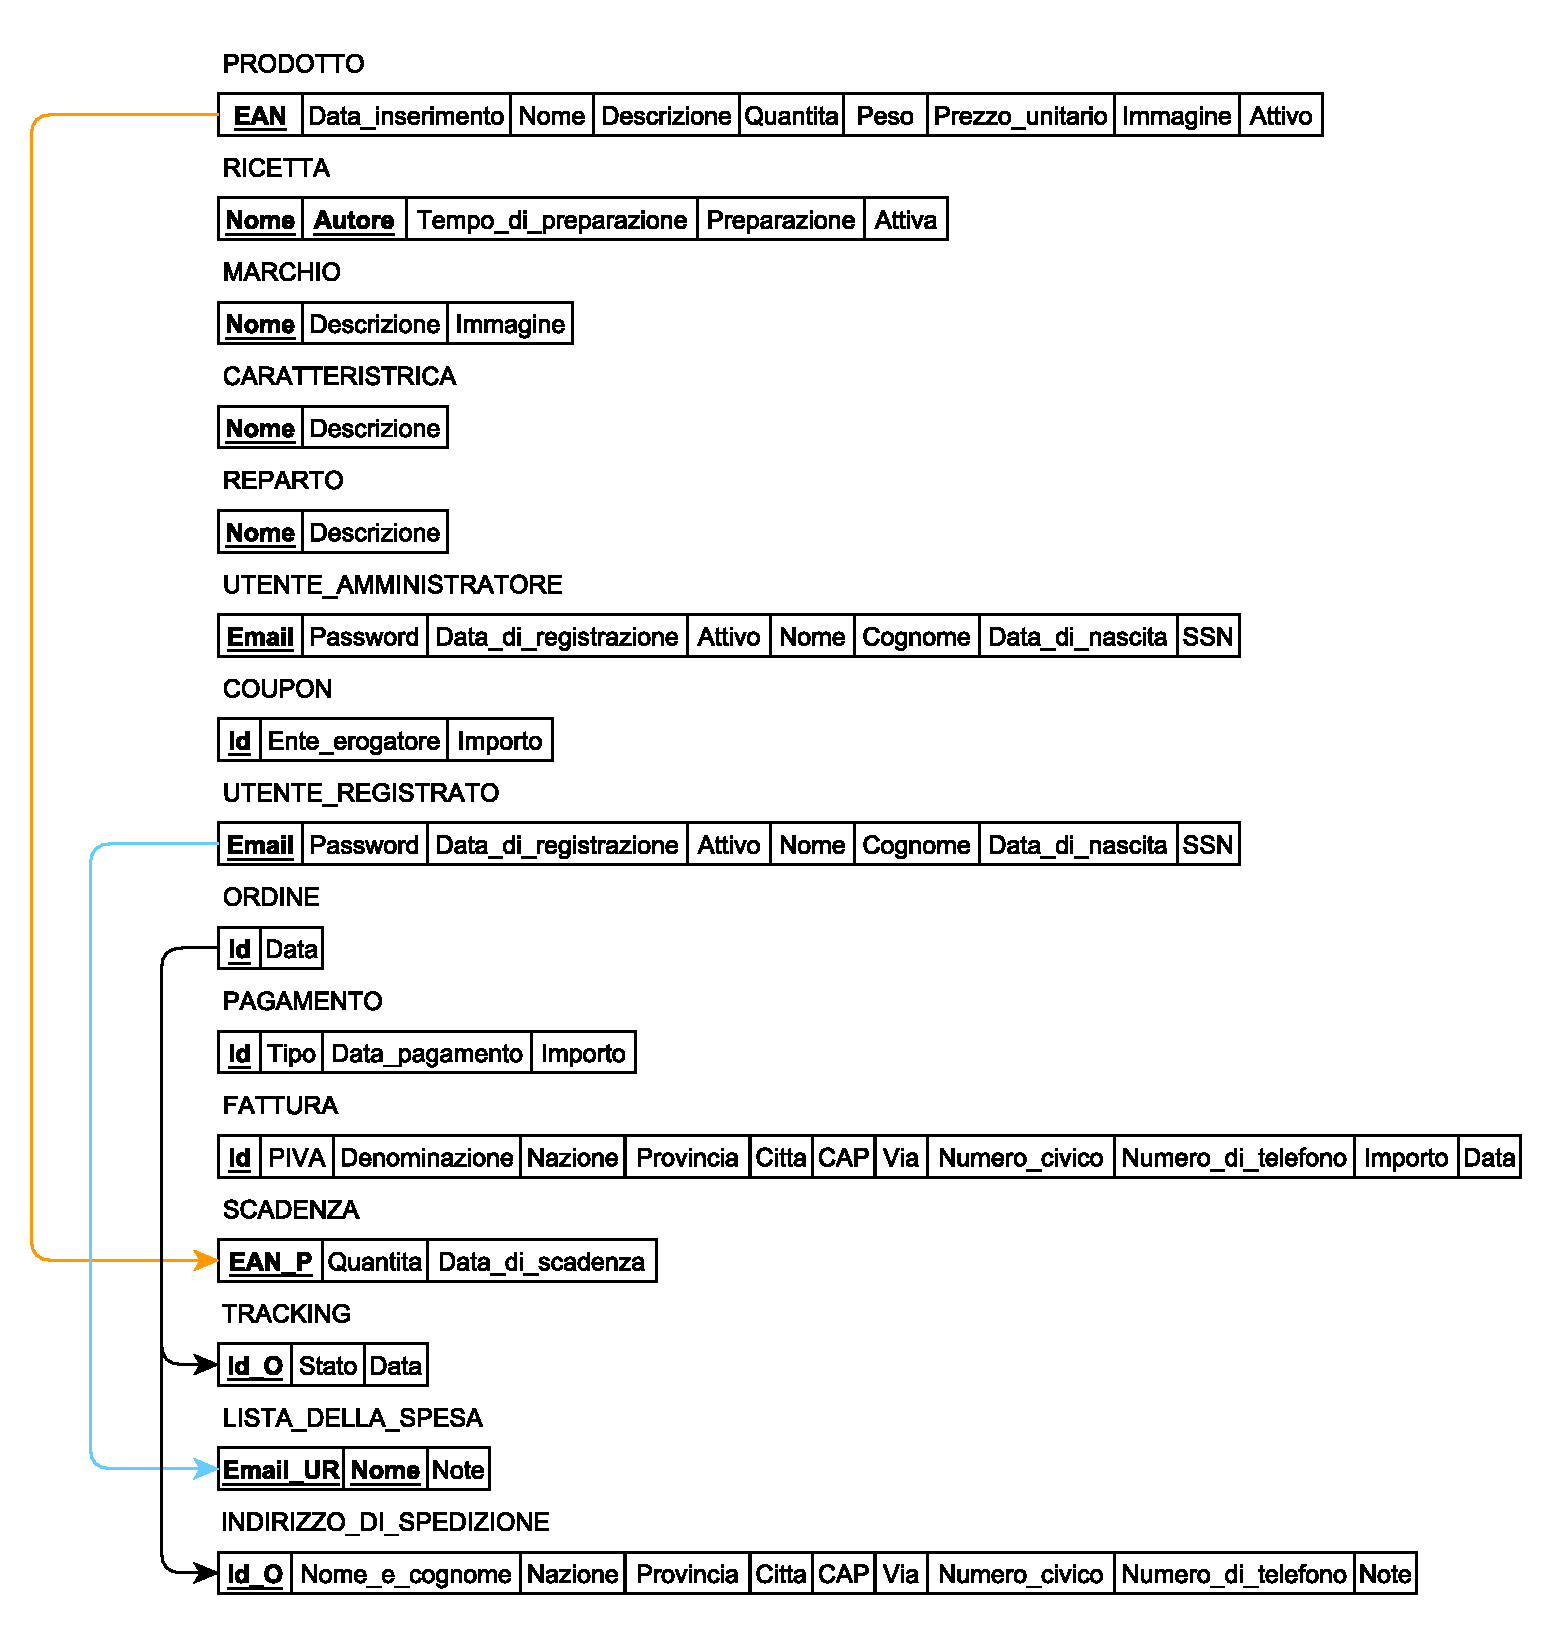
\includegraphics[width=1\textwidth]
		{immagini/traduzione-entita-deboli}
		
		\caption{Traduzione di entità deboli}
	\end{figure}
	
	\begin{figure}[h]
		\centering
		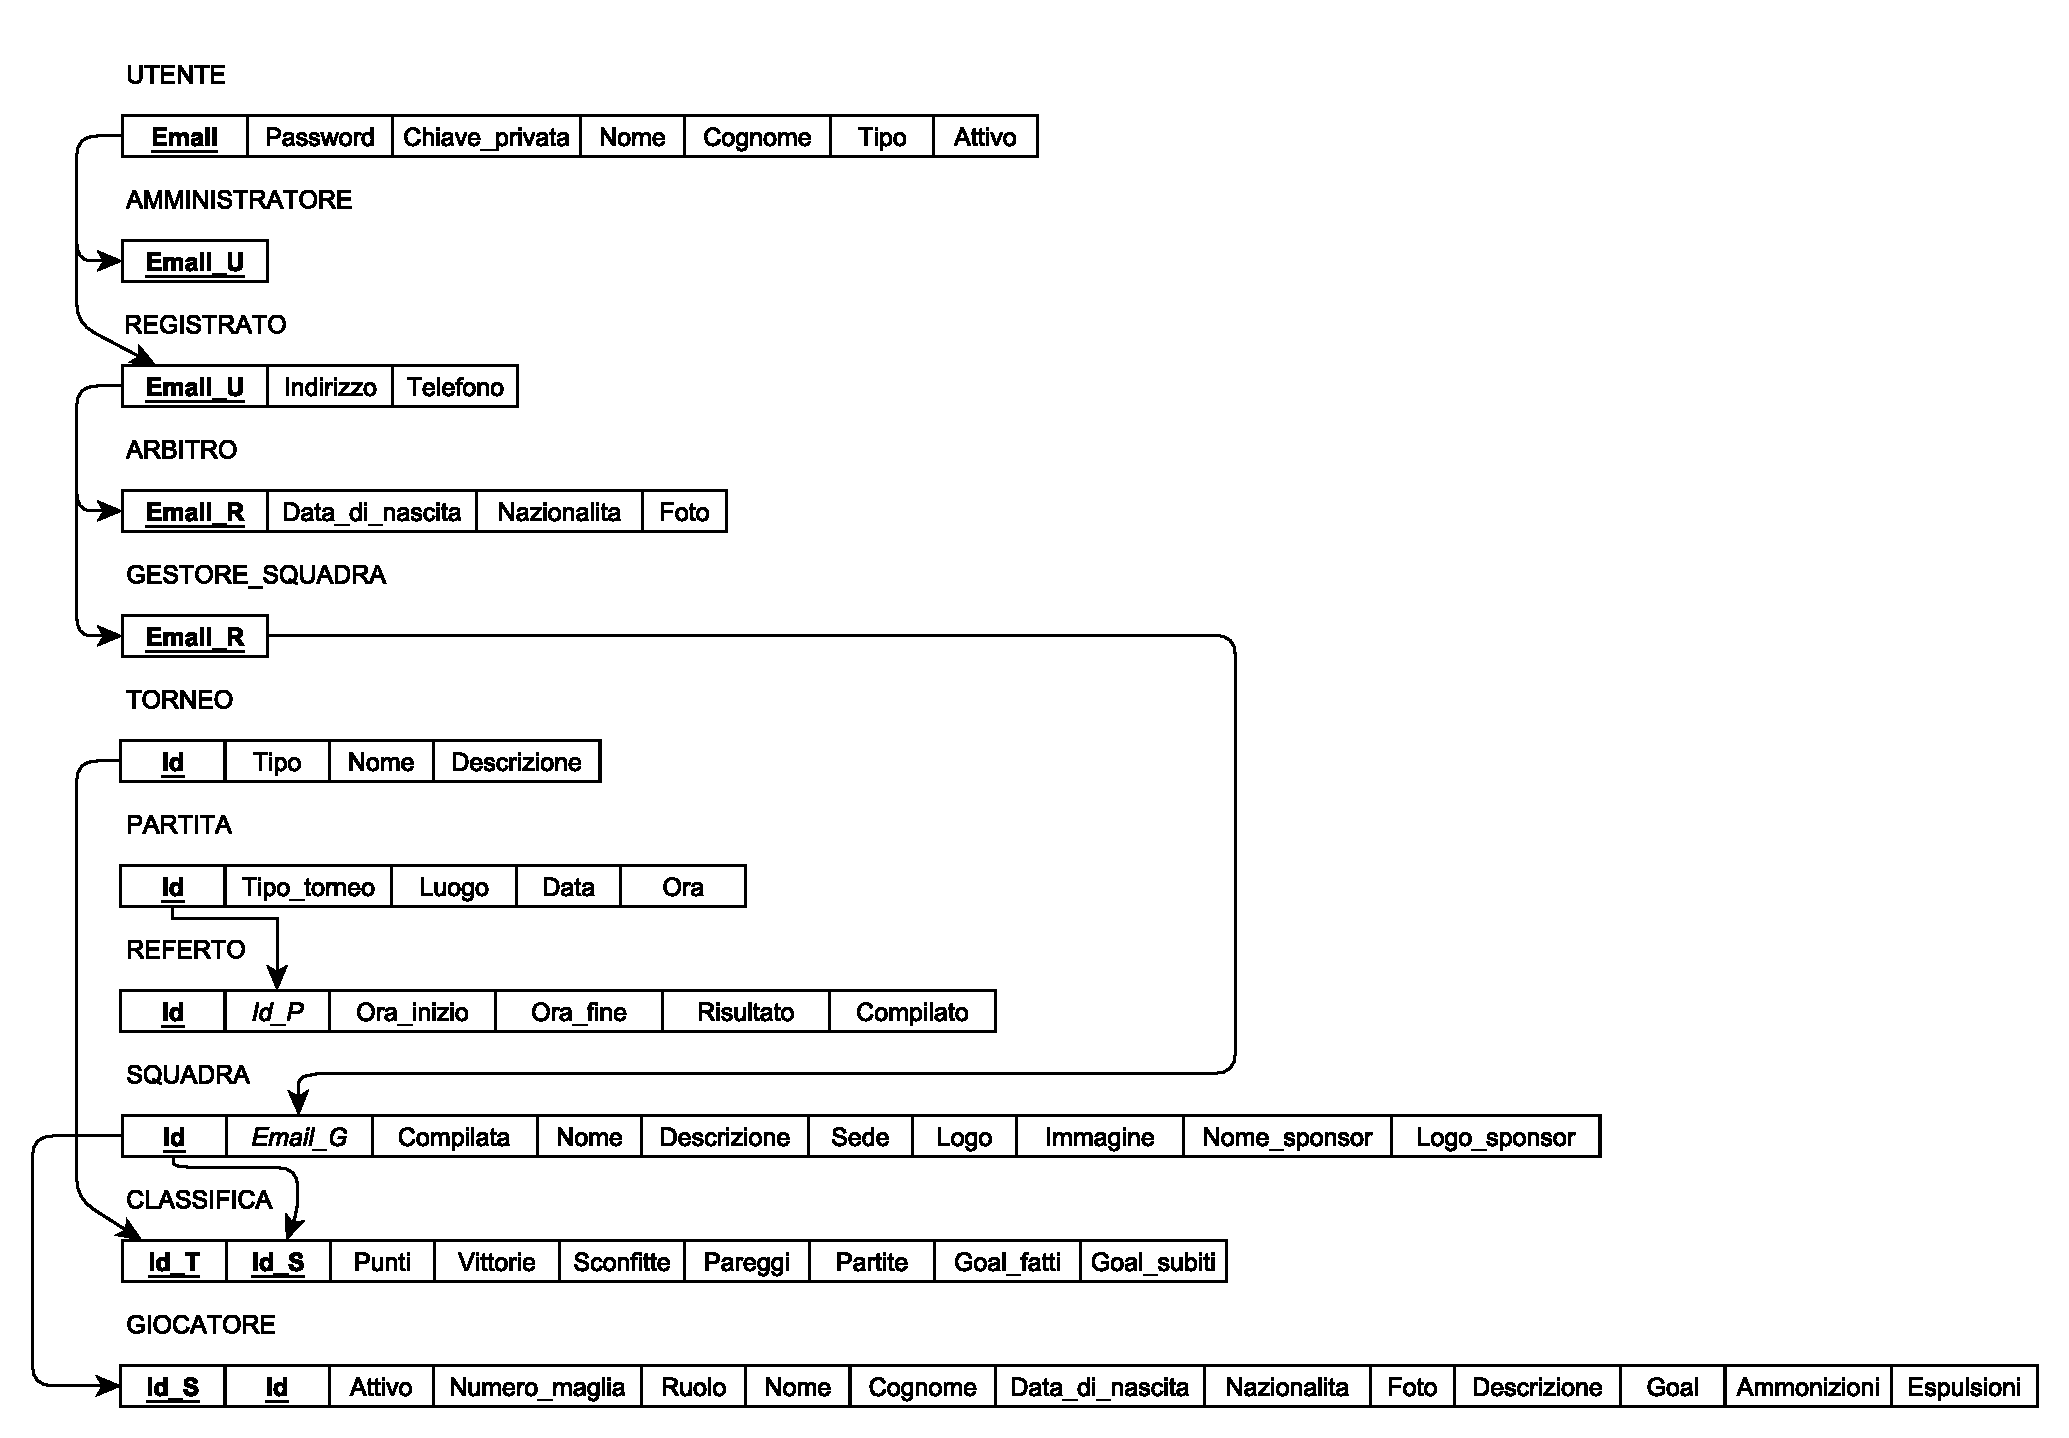
\includegraphics[width=1\textwidth]
		{immagini/traduzione-associazioni-1-1}
		
		\caption{Traduzione di associazioni binarie 1:1}
	\end{figure}
	
	\begin{figure}[h]
		\centering
		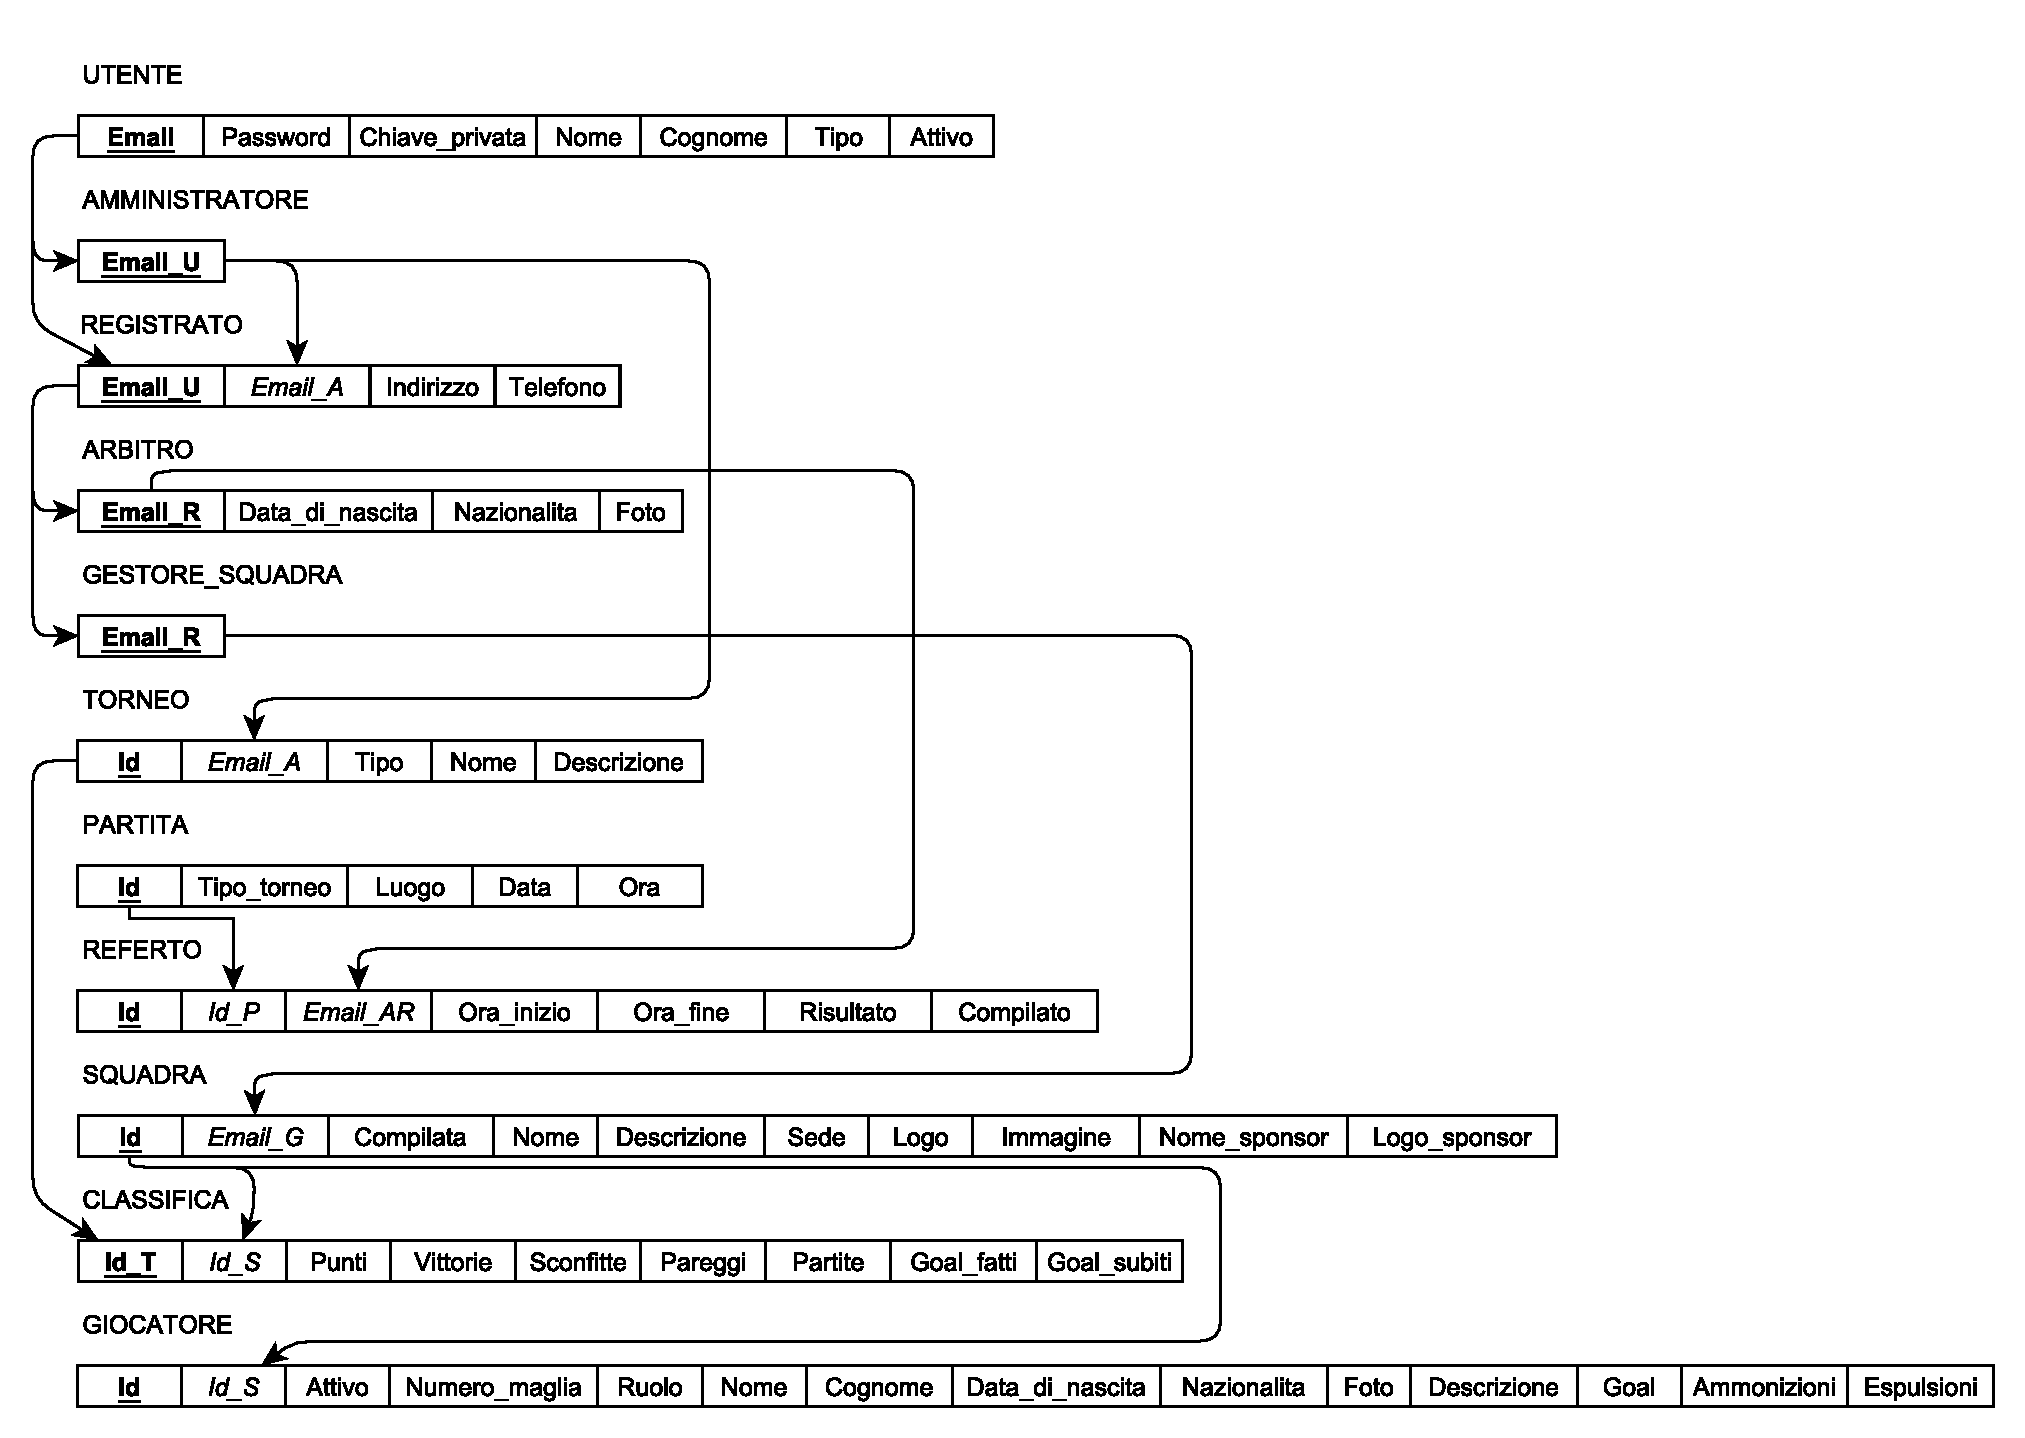
\includegraphics[width=1\textwidth]
		{immagini/traduzione-associazioni-1-N}
		
		\caption{Traduzione di associazioni binarie 1:N}
	\end{figure}
	
	\begin{figure}[h]
		\centering
		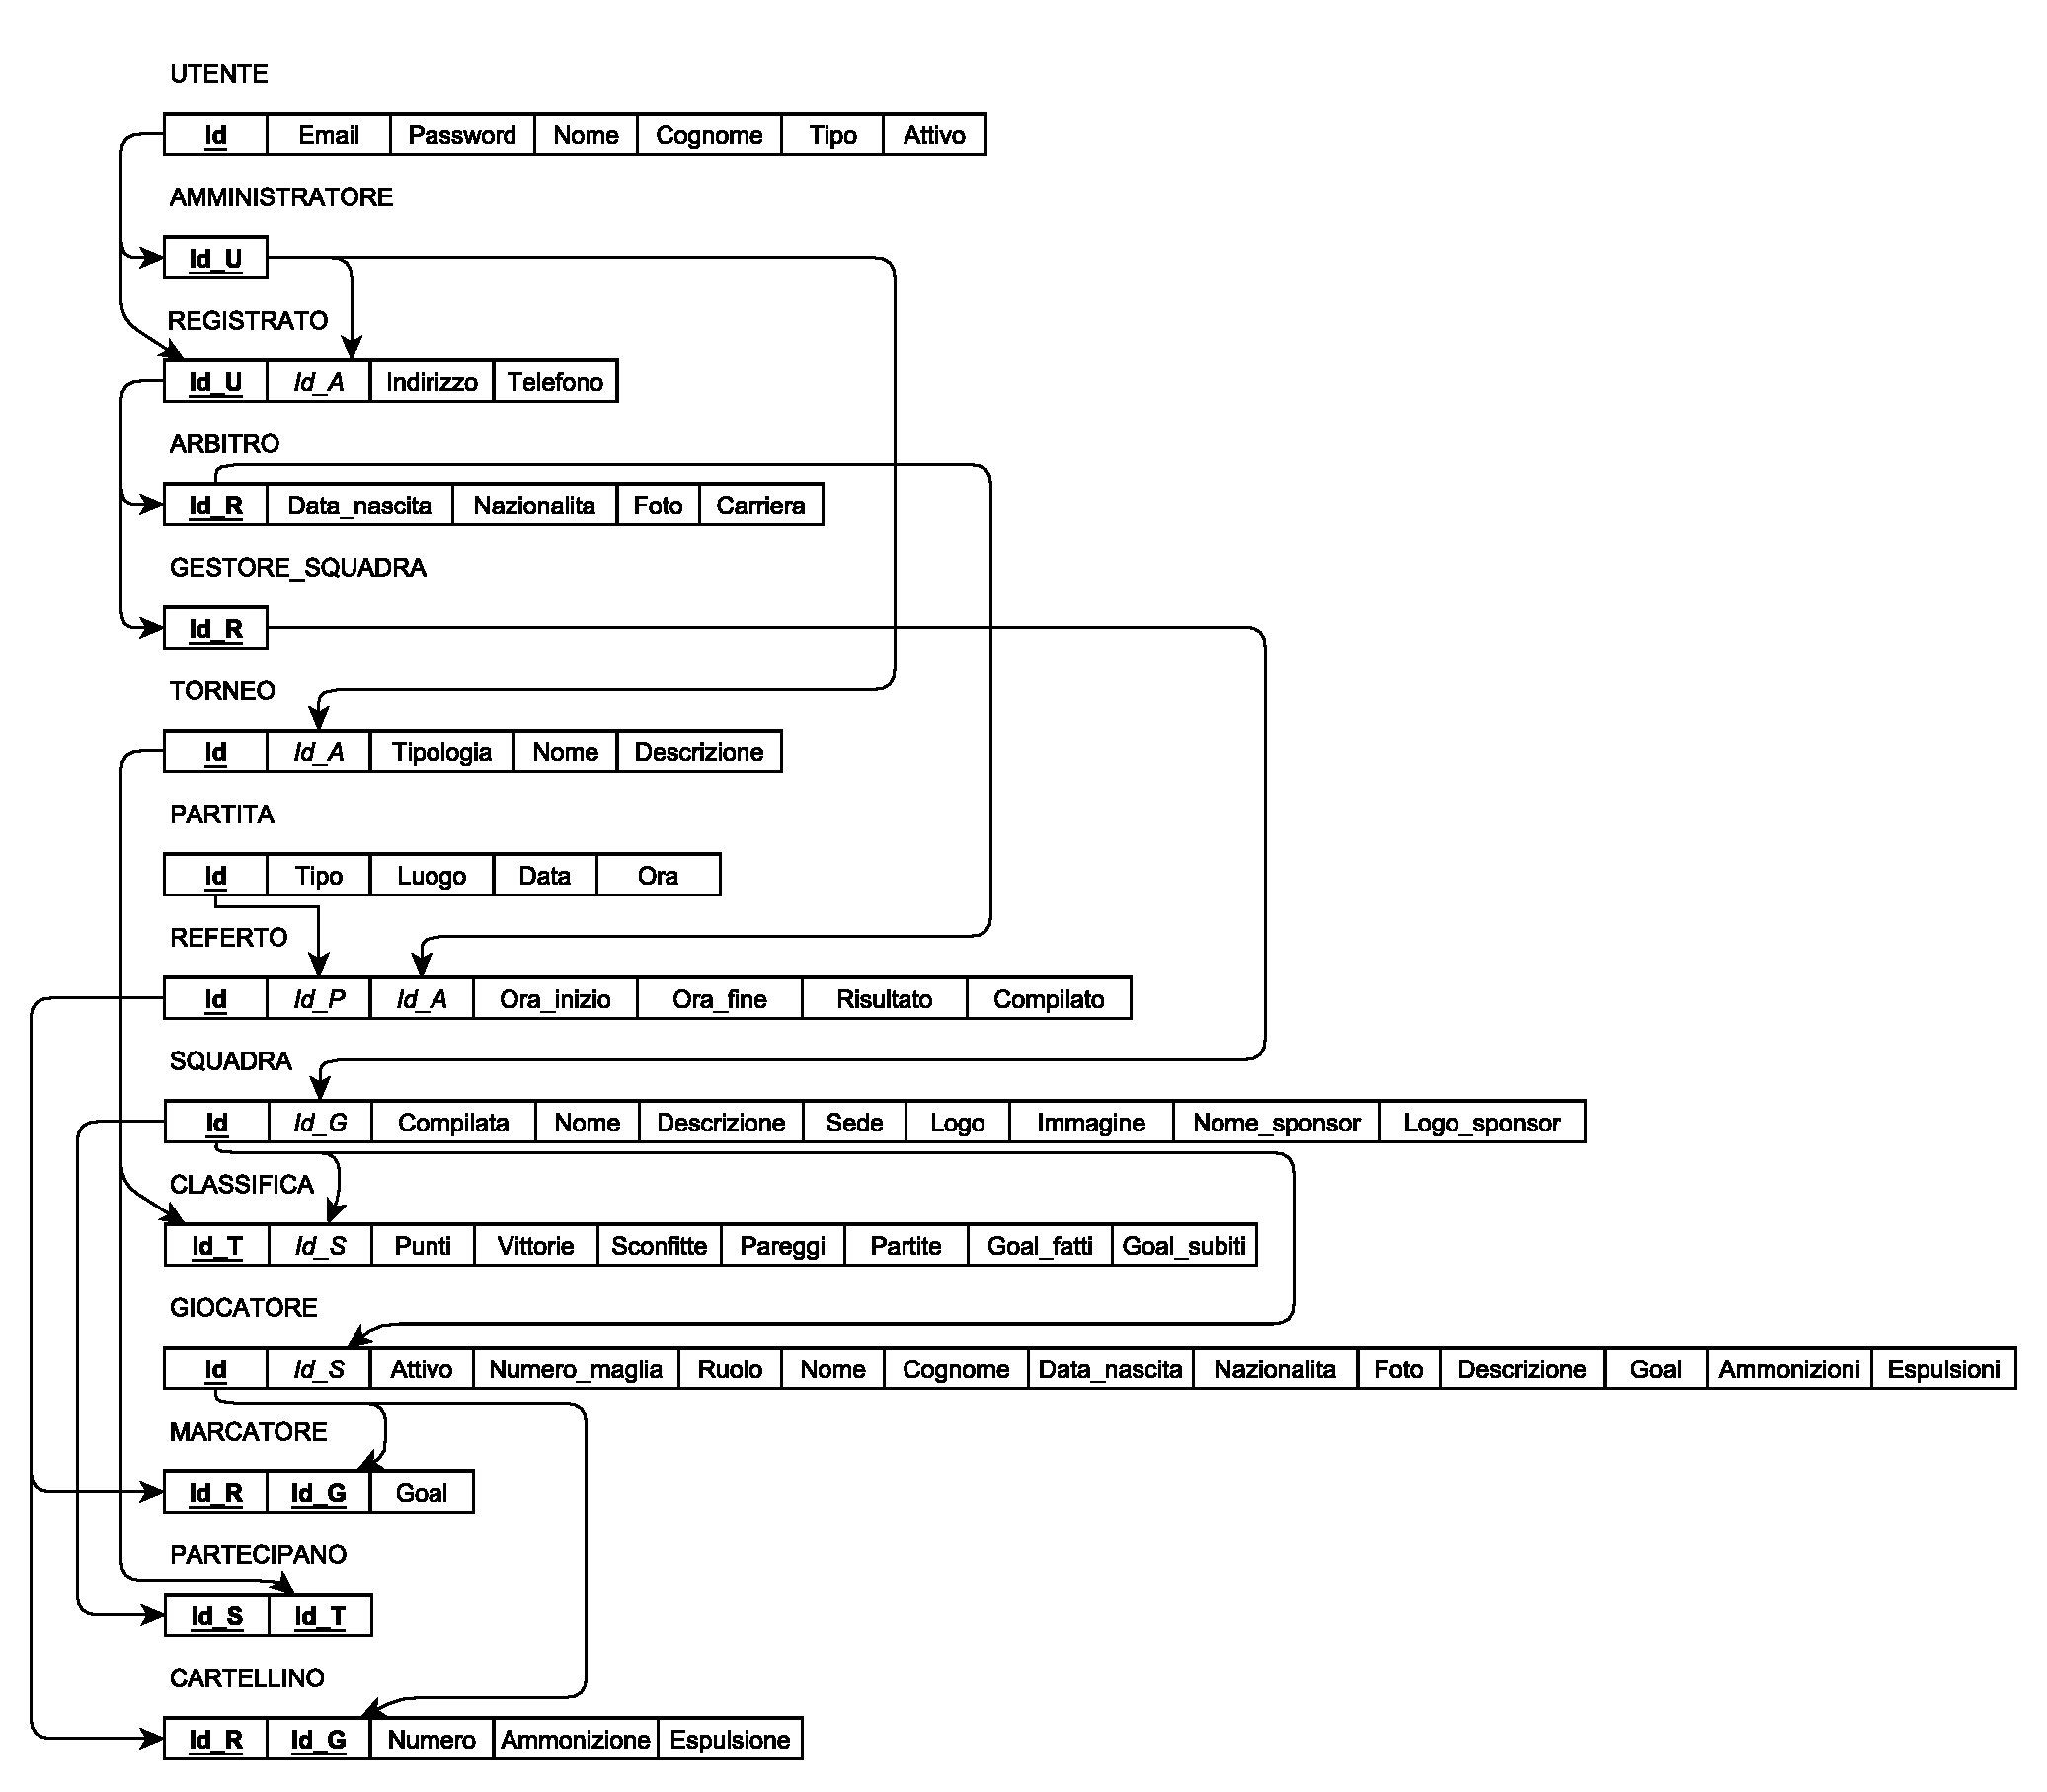
\includegraphics[width=1\textwidth]
		{immagini/traduzione-associazioni-M-N}
		
		\caption{Traduzione di associazioni binarie M:N}
		\label{f:trad-assoc-m-n}
	\end{figure}   % traduzione del modello ER in modello relazionale
% !TEX encoding = UTF-8
% !TEX TS-program = pdflatex
% !TEX root = ../Tesi.tex
% !TEX spellcheck = it-IT

%************************************************
\chapter{Normalizzazione}
\label{cap:normalizzazione}
%************************************************

\section{Elenco entità}
bla bla bla\dots{}   % normalizzazione del modello relazionale
% !TEX encoding = UTF-8
% !TEX TS-program = pdflatex
% !TEX root = ../Tesi.tex
% !TeX spellcheck = it_IT

%************************************************
\chapter{Codice SQL}
\label{cap:codice-sql}
%************************************************

\section{DDL}
Si riporta il codice SQL utilizzato per creare le tabelle che costituiscono la base di dati e i vincoli di integrità referenziale.

\subsection{Utente}
Struttura della tabella \emph{UTENTE}:

\begin{lstlisting}
CREATE TABLE IF NOT EXISTS `UTENTE` (
	`Email` VARCHAR(30) NOT NULL,
	`Password` VARCHAR(32) NOT NULL,
	`Chiave_privata` VARCHAR(32) NOT NULL,
	`Nome` VARCHAR(30) NOT NULL,
	`Cognome` VARCHAR(30) NOT NULL,
	`Tipo` VARCHAR(1) NOT NULL,
	`Attivo` BOOLEAN NOT NULL DEFAULT TRUE,
	PRIMARY KEY (`Email`)
) ENGINE = InnoDB;
\end{lstlisting}

\subsection{Amministratore}
Struttura della tabella \emph{AMMINISTRATORE}:

\begin{lstlisting}
CREATE TABLE IF NOT EXISTS `AMMINISTRATORE` (
	`Email_U` VARCHAR(30) NOT NULL,
	PRIMARY KEY (`Email_U`),
	FOREIGN KEY (`Email_U`) REFERENCES UTENTE(`Email`)
) ENGINE = InnoDB;
\end{lstlisting}

\newpage

\subsection{Registrato}
Struttura della tabella \emph{REGISTRATO}:

\begin{lstlisting}
CREATE TABLE IF NOT EXISTS `REGISTRATO` (
	`Email_U` VARCHAR(30) NOT NULL,
	`Email_A` VARCHAR(30) NOT NULL,
	`Telefono` VARCHAR(15) NOT NULL,
	`Indirizzo` VARCHAR(50) NOT NULL,
	PRIMARY KEY (`Email_U`),
	FOREIGN KEY (`Email_U`) REFERENCES UTENTE(`Email`),
	FOREIGN KEY (`Email_A`) REFERENCES AMMINISTRATORE(`Email_U`)
) ENGINE = InnoDB;
\end{lstlisting}

\subsection{Arbitro}
Struttura della tabella \emph{ARBITRO}:

\begin{lstlisting}
CREATE TABLE IF NOT EXISTS `ARBITRO` (
	`Email_R` VARCHAR(30) NOT NULL,
	`Data_di_nascita` DATE NOT NULL,
	`Nazionalita` VARCHAR(50) NOT NULL,
	`Foto` VARCHAR(50) NOT NULL,
	PRIMARY KEY (`Email_R`),
	FOREIGN KEY (`Email_R`) REFERENCES REGISTRATO(`Email_U`)
) ENGINE = InnoDB;
\end{lstlisting}

\subsection{Gestore Squadra}
Struttura della tabella \emph{GESTORE\_SQUADRA}:

\begin{lstlisting}
CREATE TABLE IF NOT EXISTS `GESTORE_SQUADRA` (
	`Email_R` VARCHAR(30) NOT NULL,
	PRIMARY KEY (`Email_R`),
	FOREIGN KEY (`Email_R`) REFERENCES REGISTRATO(`Email_U`)
) ENGINE = InnoDB;
\end{lstlisting}

\subsection{Torneo}
Struttura della tabella \emph{TORNEO}:

\begin{lstlisting}
CREATE TABLE IF NOT EXISTS `TORNEO` (
	`Id` INT UNSIGNED NOT NULL,
	`Email_A` VARCHAR(30) NOT NULL,
	`Tipo` CHAR(1) NOT NULL,
	`Nome` VARCHAR(30) NOT NULL,
	`Descrizione` TEXT(5000),
	PRIMARY KEY (`Id`),
	FOREIGN KEY (`Email_A`) REFERENCES AMMINISTRATORE(`Email_U`)
) ENGINE = InnoDB;
\end{lstlisting}

\subsection{Partita}
Struttura della tabella \emph{PARTITA}:

\begin{lstlisting}
CREATE TABLE IF NOT EXISTS `PARTITA` (
	`Id` INT UNSIGNED NOT NULL,
	`Tipo_torneo` CHAR(1) NOT NULL,
	`Luogo` VARCHAR(30) NOT NULL,
	`Data` DATE NOT NULL,
	`Ora` TIME NOT NULL,
	PRIMARY KEY (`Id`)
) ENGINE = InnoDB;
\end{lstlisting}

\subsection{Referto}
Struttura della tabella \emph{REFERTO}:

\begin{lstlisting}
CREATE TABLE IF NOT EXISTS `REFERTO` (
	`Id` INT UNSIGNED NOT NULL,
	`Id_P` INT UNSIGNED NOT NULL,
	`Email_AR` VARCHAR(30) NOT NULL,
	`Ora_inizio` TIME NOT NULL,
	`Ora_fine` TIME NOT NULL,
	`Risultato` VARCHAR(10) NOT NULL,
	`Compilato` BOOLEAN NOT NULL,
	PRIMARY KEY (`Id`),
	FOREIGN KEY (`Id_P`) REFERENCES PARTITA(`Id`),
	FOREIGN KEY (`Email_AR`) REFERENCES ARBITRO(`Email_R`)
) ENGINE = InnoDB;
\end{lstlisting}

\subsection{Squadra}
Struttura della tabella \emph{SQUADRA}:

\begin{lstlisting}
CREATE TABLE IF NOT EXISTS `SQUADRA` (
	`Id` INT UNSIGNED NOT NULL,
	`Email_G` VARCHAR(30) NOT NULL,
	`Compilata` BOOLEAN NOT NULL,
	`Nome` VARCHAR(30) NOT NULL,
	`Descrizione` TEXT(5000),
	`Sede` VARCHAR(30),
	`Logo` VARCHAR(50),
	`Immagine` VARCHAR(50),
	`Nome_sponsor` VARCHAR(30),
	`Logo_sponsor` VARCHAR(50),
	PRIMARY KEY (`Id`),
	FOREIGN KEY (`Email_G`) REFERENCES GESTORE_SQUADRA(`Email_R`)
) ENGINE = InnoDB;
\end{lstlisting}

\subsection{Classifica}
Struttura della tabella \emph{CLASSIFICA}:

\begin{lstlisting}
CREATE TABLE IF NOT EXISTS `CLASSIFICA` (
	`Id_T` INT UNSIGNED NOT NULL,
	`Id_S` INT UNSIGNED NOT NULL,
	`Punti` INT UNSIGNED DEFAULT 0,
	`Vittorie` INT UNSIGNED DEFAULT 0,
	`Sconfitte` INT UNSIGNED DEFAULT 0,
	`Pareggi` INT UNSIGNED DEFAULT 0,
	`Partite` INT UNSIGNED DEFAULT 0,
	`Goal_fatti` INT UNSIGNED DEFAULT 0,
	`Goal_subiti` INT UNSIGNED DEFAULT 0,
	PRIMARY KEY (`Id_T`, `Id_S`),
	FOREIGN KEY (`Id_T`) REFERENCES TORNEO(`Id`),
	FOREIGN KEY (`Id_S`) REFERENCES SQUADRA(`Id`)
) ENGINE = InnoDB;
\end{lstlisting}

\subsection{Giocatore}
Struttura della tabella \emph{GIOCATORE}:

\begin{lstlisting}
CREATE TABLE IF NOT EXISTS `GIOCATORE` (
	`Id` INT UNSIGNED NOT NULL,
	`Id_S` INT UNSIGNED NOT NULL,
	`Attivo` BOOLEAN DEFAULT TRUE,
	`Numero_maglia` INT UNSIGNED,
	`Ruolo` VARCHAR(50) NOT NULL,
	`Nome` VARCHAR(30) NOT NULL,
	`Cognome` VARCHAR(30) NOT NULL,
	`Data_di_nascita` DATE NOT NULL,
	`Nazionalita` VARCHAR(20) NOT NULL,
	`Foto` VARCHAR(50) NOT NULL,
	`Descrizione` TEXT(5000),
	`Goal` INT UNSIGNED DEFAULT 0,
	`Ammonizioni` INT UNSIGNED DEFAULT 0,
	`Espulsioni` INT UNSIGNED DEFAULT 0,
	PRIMARY KEY (`Id`),
	FOREIGN KEY (`Id_S`) REFERENCES SQUADRA(`Id`)
) ENGINE = InnoDB;
\end{lstlisting}

\newpage

\subsection{Marcatore}
Struttura della tabella \emph{MARCATORE}:

\begin{lstlisting}
CREATE TABLE IF NOT EXISTS `MARCATORE` (
	`Id_R` INT UNSIGNED NOT NULL,
	`Id_G` INT UNSIGNED NOT NULL,
	`Goal` INT UNSIGNED DEFAULT 0,
	PRIMARY KEY (`Id_R`, `Id_G`),
	FOREIGN KEY (`Id_R`) REFERENCES REFERTO(`Id`),
	FOREIGN KEY (`Id_G`) REFERENCES GIOCATORE(`Id`)
) ENGINE = InnoDB;
\end{lstlisting}

\subsection{Partecipano}
Struttura della tabella \emph{PARTECIPANO}:

\begin{lstlisting}
CREATE TABLE IF NOT EXISTS `PARTECIPANO` (
	`Id_S` INT UNSIGNED NOT NULL,
	`Id_T` INT UNSIGNED NOT NULL,
	PRIMARY KEY (`Id_S`, `Id_T`),
	FOREIGN KEY (`Id_S`) REFERENCES SQUADRA(`Id`),
	FOREIGN KEY (`Id_T`) REFERENCES TORNEO(`Id`)
) ENGINE = InnoDB;
\end{lstlisting}

\subsection{Cartellino}
Struttura della tabella \emph{CARTELLINO}:

\begin{lstlisting}
CREATE TABLE IF NOT EXISTS `CARTELLINO` (
	`Id_R` INT UNSIGNED NOT NULL,
	`Id_G` INT UNSIGNED NOT NULL,
	`Numero` INT UNSIGNED DEFAULT 0,
	`Ammonizione` BOOLEAN,
	`Espulsione` BOOLEAN,
	PRIMARY KEY (`Id_R`, `Id_G`),
	FOREIGN KEY (`Id_R`) REFERENCES REFERTO(`Id`),
	FOREIGN KEY (`Id_G`) REFERENCES GIOCATORE(`Id`)
) ENGINE = InnoDB;
\end{lstlisting}

\newpage

\subsection{Scelto}
Struttura della tabella \emph{SCELTO}:

\begin{lstlisting}
CREATE TABLE IF NOT EXISTS `SCELTO` (
	`Id_P` INT UNSIGNED NOT NULL,
	`Email_AR` VARCHAR(30) NOT NULL,
	`Email_A` VARCHAR(30) NOT NULL,
	PRIMARY KEY (`Id_P`, `Email_AR`, `Email_A`),
	FOREIGN KEY (`Id_P`) REFERENCES PARTITA(`Id`),
	FOREIGN KEY (`Email_AR`) REFERENCES ARBITRO(`Email_R`),
	FOREIGN KEY (`Email_A`) REFERENCES AMMINISTRATORE(`Email_U`)
) ENGINE = InnoDB;
\end{lstlisting}

\subsection{Formazione}
Struttura della tabella \emph{FORMAZIONE}:

\begin{lstlisting}
CREATE TABLE IF NOT EXISTS `FORMAZIONE` (
	`Id_R` INT UNSIGNED NOT NULL,
	`Id_S` INT UNSIGNED NOT NULL,
	`Id_G` INT UNSIGNED NOT NULL,
	`Riserva` BOOLEAN NOT NULL,
	PRIMARY KEY (`Id_R`, `Id_S`, `Id_G`),
	FOREIGN KEY (`Id_R`) REFERENCES REFERTO(`Id`),
	FOREIGN KEY (`Id_S`) REFERENCES SQUADRA(`Id`),
	FOREIGN KEY (`Id_G`) REFERENCES GIOCATORE(`Id`)
) ENGINE = InnoDB;
\end{lstlisting}

\subsection{Giocano}
Struttura della tabella \emph{GIOCANO}:

\begin{lstlisting}
CREATE TABLE IF NOT EXISTS `GIOCANO` (
	`Id_P` INT UNSIGNED NOT NULL,
	`Id_S1` INT UNSIGNED NOT NULL,
	`Id_S2` INT UNSIGNED NOT NULL,
	`Id_T` INT UNSIGNED NOT NULL,
	`Nome_partita` VARCHAR(30) NOT NULL,
	PRIMARY KEY (`Id_P`, `Id_S1`, `Id_S2`, `Id_T`),
	FOREIGN KEY (`Id_P`) REFERENCES PARTITA(`Id`),
	FOREIGN KEY (`Id_S1`) REFERENCES SQUADRA(`Id`),
	FOREIGN KEY (`Id_S2`) REFERENCES SQUADRA(`Id`),
	FOREIGN KEY (`Id_T`) REFERENCES TORNEO(`Id`)
) ENGINE = InnoDB;
\end{lstlisting}

\section{Interrogazioni}
Tra le molte interrogazioni utilizzate dall'applicazione web riguardo il database precedente si riportano quelle che meritano un commento.

\subsection{INSERT}

\subsubsection*{Inserimento arbitro}

\begin{lstlisting}
UPDATE arbitro
SET 
Foto='Conversion.getDatabaseString(foto)', data_n='Conversion.getDatabaseString(data_n)',
Nazionalita='Conversion.getDatabaseString(nazionalita)', Carriera='Conversion.getDatabaseString(carriera)'
WHERE SSN=(SELECT SSN FROM utente WHERE email='"+Conversion.getDatabaseString(email)')
\end{lstlisting}

\subsection*{Eliminazione di un utente dall'applicazione}
L'amministratore ha la possibilità di togliere i privilegi di accesso all'applicazione ad un utente registrato. In realtà non viene eliminato dal database ma viene solo cambiata la sua visibilità attraverso l'attributo \emph{Attivo}.

\begin{lstlisting}
UPDATE utente
SET flag='N' 
WHERE  email='Conversion.getDatabaseString(email)'
\end{lstlisting}


\subsection*{Inserimento dei marcatori di una partita}
Nella creazione del referto viene utilizzata questa query per inserire in una tabella tutti i giocatori che hanno segnato dei goal nella partita a cui fa riferimento il referto. Una cosa simile è stata fatta per la cartella Cartellini.

\begin{lstlisting}
INSERT INTO marcatori (ID_Referto, SSN_Giocatore, Goal) 
VALUES ('Conversion.getDatabaseString(""+IDReferto)', 'Conversion.getDatabaseString(""+SSNGiocatore)', 'Conversion.getDatabaseString(""+goal)')
\end{lstlisting}

\subsection{UPDATE}

\subsection*{Primo accesso all'applicazione del gestore di una squadra}
Primo accesso all'applicazione del gestore di una squadra

\begin{lstlisting}
UPDATE squadra
SET    Nome_squadra = 'Conversion.getDatabaseString(nomeSquadra)',
Logo_squadra = Conversion.getDatabaseString(logoSquadra),
Immagine_squadra = 'Conversion.getDatabaseString(immagine Squadra)',
Nome_sponsor = 'Conversion.getDatabaseString(nomeSponsor)',
Logo_sponsor = 'Conversion.getDatabaseString(logoSponsor)',
Sede = 'Conversion.getDatabaseString(sede)',
Descrizione = 'Conversion.getDatabaseString(descrizione)',
flag = 'Y'
WHERE  SSN_Gestore = 'Conversion.getDatabaseString(""+gestore)'
\end{lstlisting}

\subsection*{Inserimento di un nuovo arbitro}
L'amministratore ha la possibilità di inserire un nuovo arbitro, a esso gli viene attribuita la lettera ``R'' (dall'inglese Refree) nell'attributo \emph{Tipo}. Le query sono tre perchè l'arbitro è un registrato che a sua volta è un cliente.

\subsubsection*{Inserimento utente}

\begin{lstlisting}
UPDATE utente
SET 
flag='Y', type='R', Nome='Conversion.getDatabaseString(nome)', Cognome='Conversion.getDatabaseString(cognome)',
Password='Conversion.getDatabaseString(password)'
WHERE email='Conversion.getDatabaseString(email)'
\end{lstlisting}

\subsubsection*{Inserimento registrato}

\begin{lstlisting}
UPDATE registrato
SET 
Telefono='Conversion.getDatabaseString(telefono)', Indirizzo='Conversion.getDatabaseString(indirizzo)',
SSN_Admin='Conversion.getDatabaseString(""+Admin)'
WHERE SSN=(SELECT SSN              FROM utente             WHERE email='Conversion.getDatabaseString(email)')
\end{lstlisting}

\subsection{SELECT}

\subsection*{Ricerca partite senza nessun arbitro}

\begin{lstlisting}
SELECT p.Data_partita, R.ID_Referto,g., r.flagRef, t.Nome AS nomeTorneo
FROM referto AS r, giocano AS g, torneo AS t, partita AS p
WHERE 	r.flagRef='N' AND
G.ID_Partita=r.ID_Partita AND
g.ID_Torneo=t.ID_Torneo AND
r.ID_Partita=p.ID_Partita AND
g.ID_Partita=p.ID_Partita AND
(G.ID_SquadraA IN
(SELECT ID_SQUADRA
FROM SQUADRA 
WHERE ssn_gESTORE='"+Conversion.getDatabaseString(""+gestore)  AND
ID_Squadra<>'0')
OR G.ID_SquadraB IN
(SELECT ID_SQUADRA
FROM SQUADRA
WHERE ssn_gESTORE='"+Conversion.getDatabaseString(""+gestore) AND
ID_Squadra<>'0')) 
AND R.ID_Referto NOT IN
(SELECT ID_Referto
FROM formazione 
WHERE ID_Squadra=(SELECT ID_Squadra
FROM squadra
WHERE SSN_Gestore='"+Conversion.getDatabaseString(""+gestore)))
ORDER BY ID_Referto
\end{lstlisting}

\subsection*{Ricerca dei referti assegnati ad un arbitro da un amministratore}
Quando l'amministratore del sistema deve sorteggiare un arbitro per una determinata partita riguardante una certa fase di un determinato torneo, deve poter visualizzare soltanto gli incontri per cui il sorteggio non sia già stato effettuato.

\begin{lstlisting}
SELECT 	Ref.ID_Referto, Ref.Risultato, Ref.Ora_inizio,
Ref.Ora_fine, Ref.ID_Partita, Ref.Risultato,
Ref.flagRef,U.Nome AS nomeArbitro,
U.cognome AS cognomeArbitro,T.ID_Torneo,
T.tipologia as tipoTorneo, T.Nome as nomeTorneo,
P.Data_Partita, P.Luogo
FROM 	referto AS Ref, utente AS U, registrato AS Reg,
giocano as G, torneo as T, partita as P
WHERE	U.Flag='Y' AND U.type='R' AND
U.SSN=Reg.SSN AND U.SSN=Ref.SSN_Arbitro
AND g.id_partita=Ref.ID_Partita
AND t.ID_Torneo=G.ID_Torneo
AND p.ID_Partita=G.ID_Partita
AND Reg.SSN_Admin='"+Conversion.getDatabaseString(""+Admin)'
ORDER BY Ref.ID_Referto 
\end{lstlisting}

\subsection*{Estrazione dei cartellini dei giocatori in una determinata partita}
Questa query viene utilizzata dall'utente pubblico quando va a visionare il referto relativo ad una determinata partita. Vengono estratte dalla tabella i cartellini di tutti i giocatori e le espulsioni e le ammonizioni relative ad una determinata partita. GLi \emph{Id} dei giocatori verranno poi confrontati con gli \emph{Id} dei giocatori delle due formazioni e se risultano uguali allora estraggo il flag ammonito/espulso e li visualizzo a schermo. Una query simile è stata fatta per la cartella Marcatori.

\begin{lstlisting}
SELECT g.Nome, g.Cognome, g.Foto, g.Foto, g.SSN_Gct, G.ID_Squadra, c.Flag_Ammonito as FlagAmmonito, c.Flag_Espulso as FlagEspulso
FROM giocatore AS g, cartellini_gialli AS C
WHERE C.SSN_Giocatore=G.SSN_Gct  AND C.ID_Referto='Conversion.getDatabaseString(""+IDReferto)'
AND (G.ID_Squadra='Conversion.getDatabaseString(""+IDSquadraA)' OR G.ID_Squadra='Conversion.getDatabaseString(""+IDSquadraB)')
\end{lstlisting}   % codice SQL
% !TEX encoding = UTF-8
% !TEX TS-program = pdflatex
% !TEX root = ../Tesi.tex
% !TEX spellcheck = it-IT

%************************************************
\chapter{Interfaccia grafica}
\label{cap:interfaccia-grafica}
%************************************************

\section{Elenco entità}
bla bla bla\dots{}   % interfaccia grafica
%\appendix
%% !TEX encoding = UTF-8
% !TEX TS-program = pdflatex
% !TEX root = ../Tesi.tex
% !TEX spellcheck = it-IT

%************************************************
\chapter{Dolor}
\label{cap:dolor}
%************************************************

Nam dui ligula, fringilla a, euismod sodales, sollicitudin vel, wisi. Morbi auctor lorem non justo. Nam lacus libero, pretium at, lobortis vitae, ultricies et, tellus. 

\section{Mane}
\lipsum[5]

\section{Tekel}
\lipsum[6]

\section{Fares}
Sed commodo posuere pede. Mauris ut est. Ut quis purus. Sed ac odio. Sed vehicula hendrerit sem. Duis non odio. Morbi ut dui. Sed accumsan risus eget odio. In hac habitasse platea dictumst. Pellentesque non elit. Fusce sed justo eu urna porta tincidunt. Mauris felis odio, sollicitudin sed, volutpat a, ornare ac, erat. Morbi quis dolor. Donec pellentesque, erat ac sagittis semper, nunc dui lobortis purus, quis congue purus metus dolor.
% *****************************************************************
% Materiale finale
%******************************************************************
%% !TEX encoding = UTF-8
% !TEX TS-program = pdflatex
% !TEX root = ../Tesi.tex
% !TEX spellcheck = it-IT

%*******************************************************
% Bibliografia
%*******************************************************
\cleardoublepage
\nocite{*}
\printbibliography
%% !TEX encoding = UTF-8
% !TEX TS-program = pdflatex
% !TEX root = ../Tesi.tex
% !TEX spellcheck = it-IT

%*******************************************************
% Dichiarazione
%*******************************************************
\cleardoublepage
\phantomsection
\pdfbookmark{Dichiarazione}{Dichiarazione}
\chapter*{Dichiarazione}
\thispagestyle{empty}

Lorem ipsum dolor sit amet, consectetuer adipiscing elit. Ut purus elit, vestibulum ut, placerat ac, adipiscing vitae, felis. Curabitur dictum gravida mauris. Nam arcu libero, nonummy eget, consectetuer id, vulputate a, magna. Donec vehicula augue eu neque.

Pellentesque habitant morbi tristique senectus et netus et malesuada fames ac turpis egestas. Mauris ut leo. Cras viverra metus rhoncus sem. Nulla et lectus vestibulum urna fringilla ultrices.

\bigskip
 
\noindent\textit{\myLocation, \MakeTextLowercase{\myTime}}

\smallskip

\begin{flushright}
    \begin{tabular}{m{5cm}}
        \\ \hline
        \centering\myName \\
    \end{tabular}
\end{flushright}

\end{document}